\documentclass[11pt,a4paper]{book}

\usepackage[bottom=0.9in,top=0.85in,left=1in,right=1in]{geometry}
\usepackage{microtype}
\usepackage{parskip}
\usepackage{etoolbox}    % robustify, used with bfseries in table formatting
\usepackage[usenames,dvipsnames]{xcolor}
\usepackage{textcomp}    % textquotesingle
\usepackage{graphicx}
\usepackage{tcolorbox}   % fancy frame around a figure
\usepackage{siunitx}
\usepackage{booktabs}    % toprule, midrule, bottomrule
\usepackage{minted}      % code listings
\usepackage{tikz}        % tikz and fadings used in title page
\usetikzlibrary{fadings}

\pagestyle{plain}

\setlength{\parskip}{\medskipamount}
\robustify\bfseries      % https://tex.stackexchange.com/questions/66253/siunitx-bold-single-numeric-cells

\newcommand{\BookVersionString}{Version 0.2.1}
\newcommand{\BookVersionDate}{6 July 2021}
\newcommand{\BookDownloadText}{Find the latest version at \texttt{bit.ly/hsifcb}}

% ------------------------------------------------------------- Commands & Includes


% -------------- Problem number counter, chapter, question header

\newcounter{problemnumber}

\newcommand{\chaptermacro}[1]{\chapter*{#1}
  \addcontentsline{toc}{chapter}{#1}}

\newcommand{\questionheader}[1]{\stepcounter{problemnumber}
  \section*{\theproblemnumber\quad #1}
  \addcontentsline{toc}{section}{\theproblemnumber\hspace{0.5em} #1}}

\newcommand{\questionheadercontinued}[1]{{\Large\color{RoyalPurple}
  \theproblemnumber\quad #1\quad\textit{continued\dots}
  \vspace{18pt}
}}

% -------------- IN, OUT, colours, future reference, note

\newcommand{\IN}{\texttt{IN}}
\newcommand{\OUT}{\texttt{OUT}}

\definecolor{MyGrey}{gray}{0.45}
\newcommand{\grey}[1]{{\color{MyGrey}#1}}

\newcommand{\futurereference}[1]{\textbf{\color{Plum}Ref: #1}}
\newcommand{\note}[1]{\textbf{\color{Orchid}Note: #1}}

% -------------- Question, Input, Output, Sample, Explanation, ......

\newcommand{\Question}{\textbf{\color{purple}Question}\quad}
\newcommand{\Note}{\vspace{6pt}\textbf{\color{purple}Note}\quad}
\newcommand{\Input}{\vspace{6pt}\textbf{\color{purple}Input}\quad}
\newcommand{\Output}{\vspace{6pt}\textbf{\color{purple}Output}\quad}
\newcommand{\Sample}{\vspace{6pt}\textbf{\color{purple}Sample}\quad}
\newcommand{\Explanation}{\vspace{6pt}\textbf{\color{purple}Explanation}\quad}
\newcommand{\Scratch}{\vspace{6pt}\textbf{\color{purple}Scratch}\quad}
\newcommand{\Solution}{\vspace{6pt}\textbf{\color{purple}Solution}\quad}
\newcommand{\Notes}{\vspace{6pt}\textbf{\color{purple}Notes}\quad}
\newcommand{\Afterword}{\vspace{6pt}\textbf{\color{purple}Afterword}\quad}
\newcommand{\Running}{\vspace{6pt}\textbf{\color{purple}Running the code}\quad}
\newcommand{\Hint}{\vspace{6pt}\textbf{\color{purple}Hint}\quad}

% -------------- workedexample, stronghint

\newcommand{\workedexample}{{\color{purple}(worked example)}}
\newcommand{\stronghint}{{\color{purple}(strongly hinted)}}

% -------------- Python code listings

\newminted{python}{xleftmargin=2cm, linenos}
\newmintinline[pycode]{python}{}

% -------------- \sample and its encompassing minipagestwo and minipagesthree

%% % <hack> Frame all minipages, to aid in layout. Comment out when not wanted,
%% %        which is most of the time.
%% \let\minipagebak\minipage
%% \let\endminipagebak\endminipage
%% \newsavebox\TestBox
%% \renewenvironment{minipage}[2][]
%% {\begin{lrbox}{\TestBox}\begin{minipagebak}[#1]{#2}}
%% {\end{minipagebak}\end{lrbox}\fbox{\usebox{\TestBox}}}
%% % </hack>

\newcommand{\sample}[4]{%
  \begin{minipage}[t]{1.2cm}
    ~~~
  \end{minipage} %
  \begin{minipage}[t]{#1\textwidth}
    \textbf{IN}\\[3pt]
    \ttfamily
    #2
  \end{minipage} %
  \begin{minipage}[t]{#3\textwidth}
    \textbf{OUT}\\[3pt]
    \ttfamily
    #4
  \end{minipage}}

\newcommand{\minipagestwo}[2]{
  \begin{minipage}[t]{0.5\textwidth}
    #1
  \end{minipage} %
  \begin{minipage}[t]{0.5\textwidth}
    #2
  \end{minipage}}

\newcommand{\minipagesthree}[3]{
  \begin{minipage}[t]{0.33333\textwidth}
    #1
  \end{minipage} %
  \begin{minipage}[t]{0.33333\textwidth}
    #2
  \end{minipage} %
  \begin{minipage}[t]{0.33333\textwidth}
    #3
  \end{minipage}}

% -------------- environment for inline tables
%                  inlinetable  - bigkip above and below
%                  inlinetable* - medskip above, bigskip below

\newenvironment{inlinetable}{
  \bigskip
  \begin{center}
}{
  \end{center}
  \bigskip
}

\newenvironment{inlinetable*}{
  \medskip
  \begin{center}
}{
  \end{center}
  \bigskip
}



% DONE

% By the way, the purpose of this is to limit the chapters that get processed in the book.
% So by commenting some of these now, I'll get a slimmed down book that reflects what I'm
% working on.

\includeonly{
  000-Titlepage,
  000-Introduction,
  100-overview,
  100-who-is-the-tallest-1,
  100-the-cheapest-tv,
  100-shopping-1,
  100-jogging-1,
  100-who-is-the-tallest-2,
  100-a-fair-wage-1,
  200-overview,
  200-shopping-2,
  200-sum-of-squares,
  200-check-the-invite-list,
  200-scrabble-tally,
  200-buried-treasure,
  200-area-calculator,
  200-drought,
  200-cute-numbers,
  200-even-numbers-for-photos-1,
  200-even-numbers-for-photos-2,
  300-overview,
  300-jogging-2,
  300-collatz-1,
  400-overview,
  400-shopping-3,
  400-a-fair-wage-2,
  400-addition-carry,
  500-overview,
  500-golf-1,
  500-half-full-flat-white,
  500-one-day-ill-be-rich,
  500-profit-and-loss-1,
  500-profit-and-loss-2,
  500-collatz-2,
  500-underreporting,
  500-sales-stars,
  500-percentage-profit,
  500-high-wire-walk,
  600-overview,
  600-golf-2,
  600-find-a-word-1,
  600-find-a-word-2,
  999-document-history,
}

% ==================================== Document ====================================

\begin{document}

% ----------------------------------------------- Title page, Contents, Introduction

\newgeometry{left=1in, right=1in,top=1in, bottom=0in}
{

\DeclareFixedFont{\titlefont}{T1}{ppl}{b}{}{0.5in}
\DeclareFixedFont{\subtitlefont}{T1}{ppl}{m}{it}{0.4in}
\DeclareFixedFont{\authorfont}{T1}{ppl}{sb}{}{0.3in}
\DeclareFixedFont{\versionfont}{T1}{ppl}{}{}{0.2in}
\DeclareFixedFont{\downloadfont}{T1}{ppl}{}{}{0.15in}

\definecolor{mytan}{HTML}{F6D5A8}
\pagecolor{mytan}

\colorlet{greytitle1}{black!95!}
\colorlet{greytitle2}{black!65!}
\colorlet{greytitle3}{black!75!}

\thispagestyle{empty}
\begin{flushright}
  \color{greytitle1}
  \titlefont High School Informatics\\[9pt] 
  \color{greytitle2}
  \subtitlefont for complete beginners\\[24pt]
  \color{greytitle3}
  \authorfont Gavin Sinclair
  \vfill
  \versionfont \BookVersionString \\[6pt] \BookVersionDate \\[12pt]
  \color{greytitle2}
  \downloadfont \BookDownloadText
  \vfill
\end{flushright}

\begin{center}
  \begin{tikzpicture}
    \node[scope fading=north, inner sep=0pt, outer sep=0pt]{
       \makebox[\textwidth]{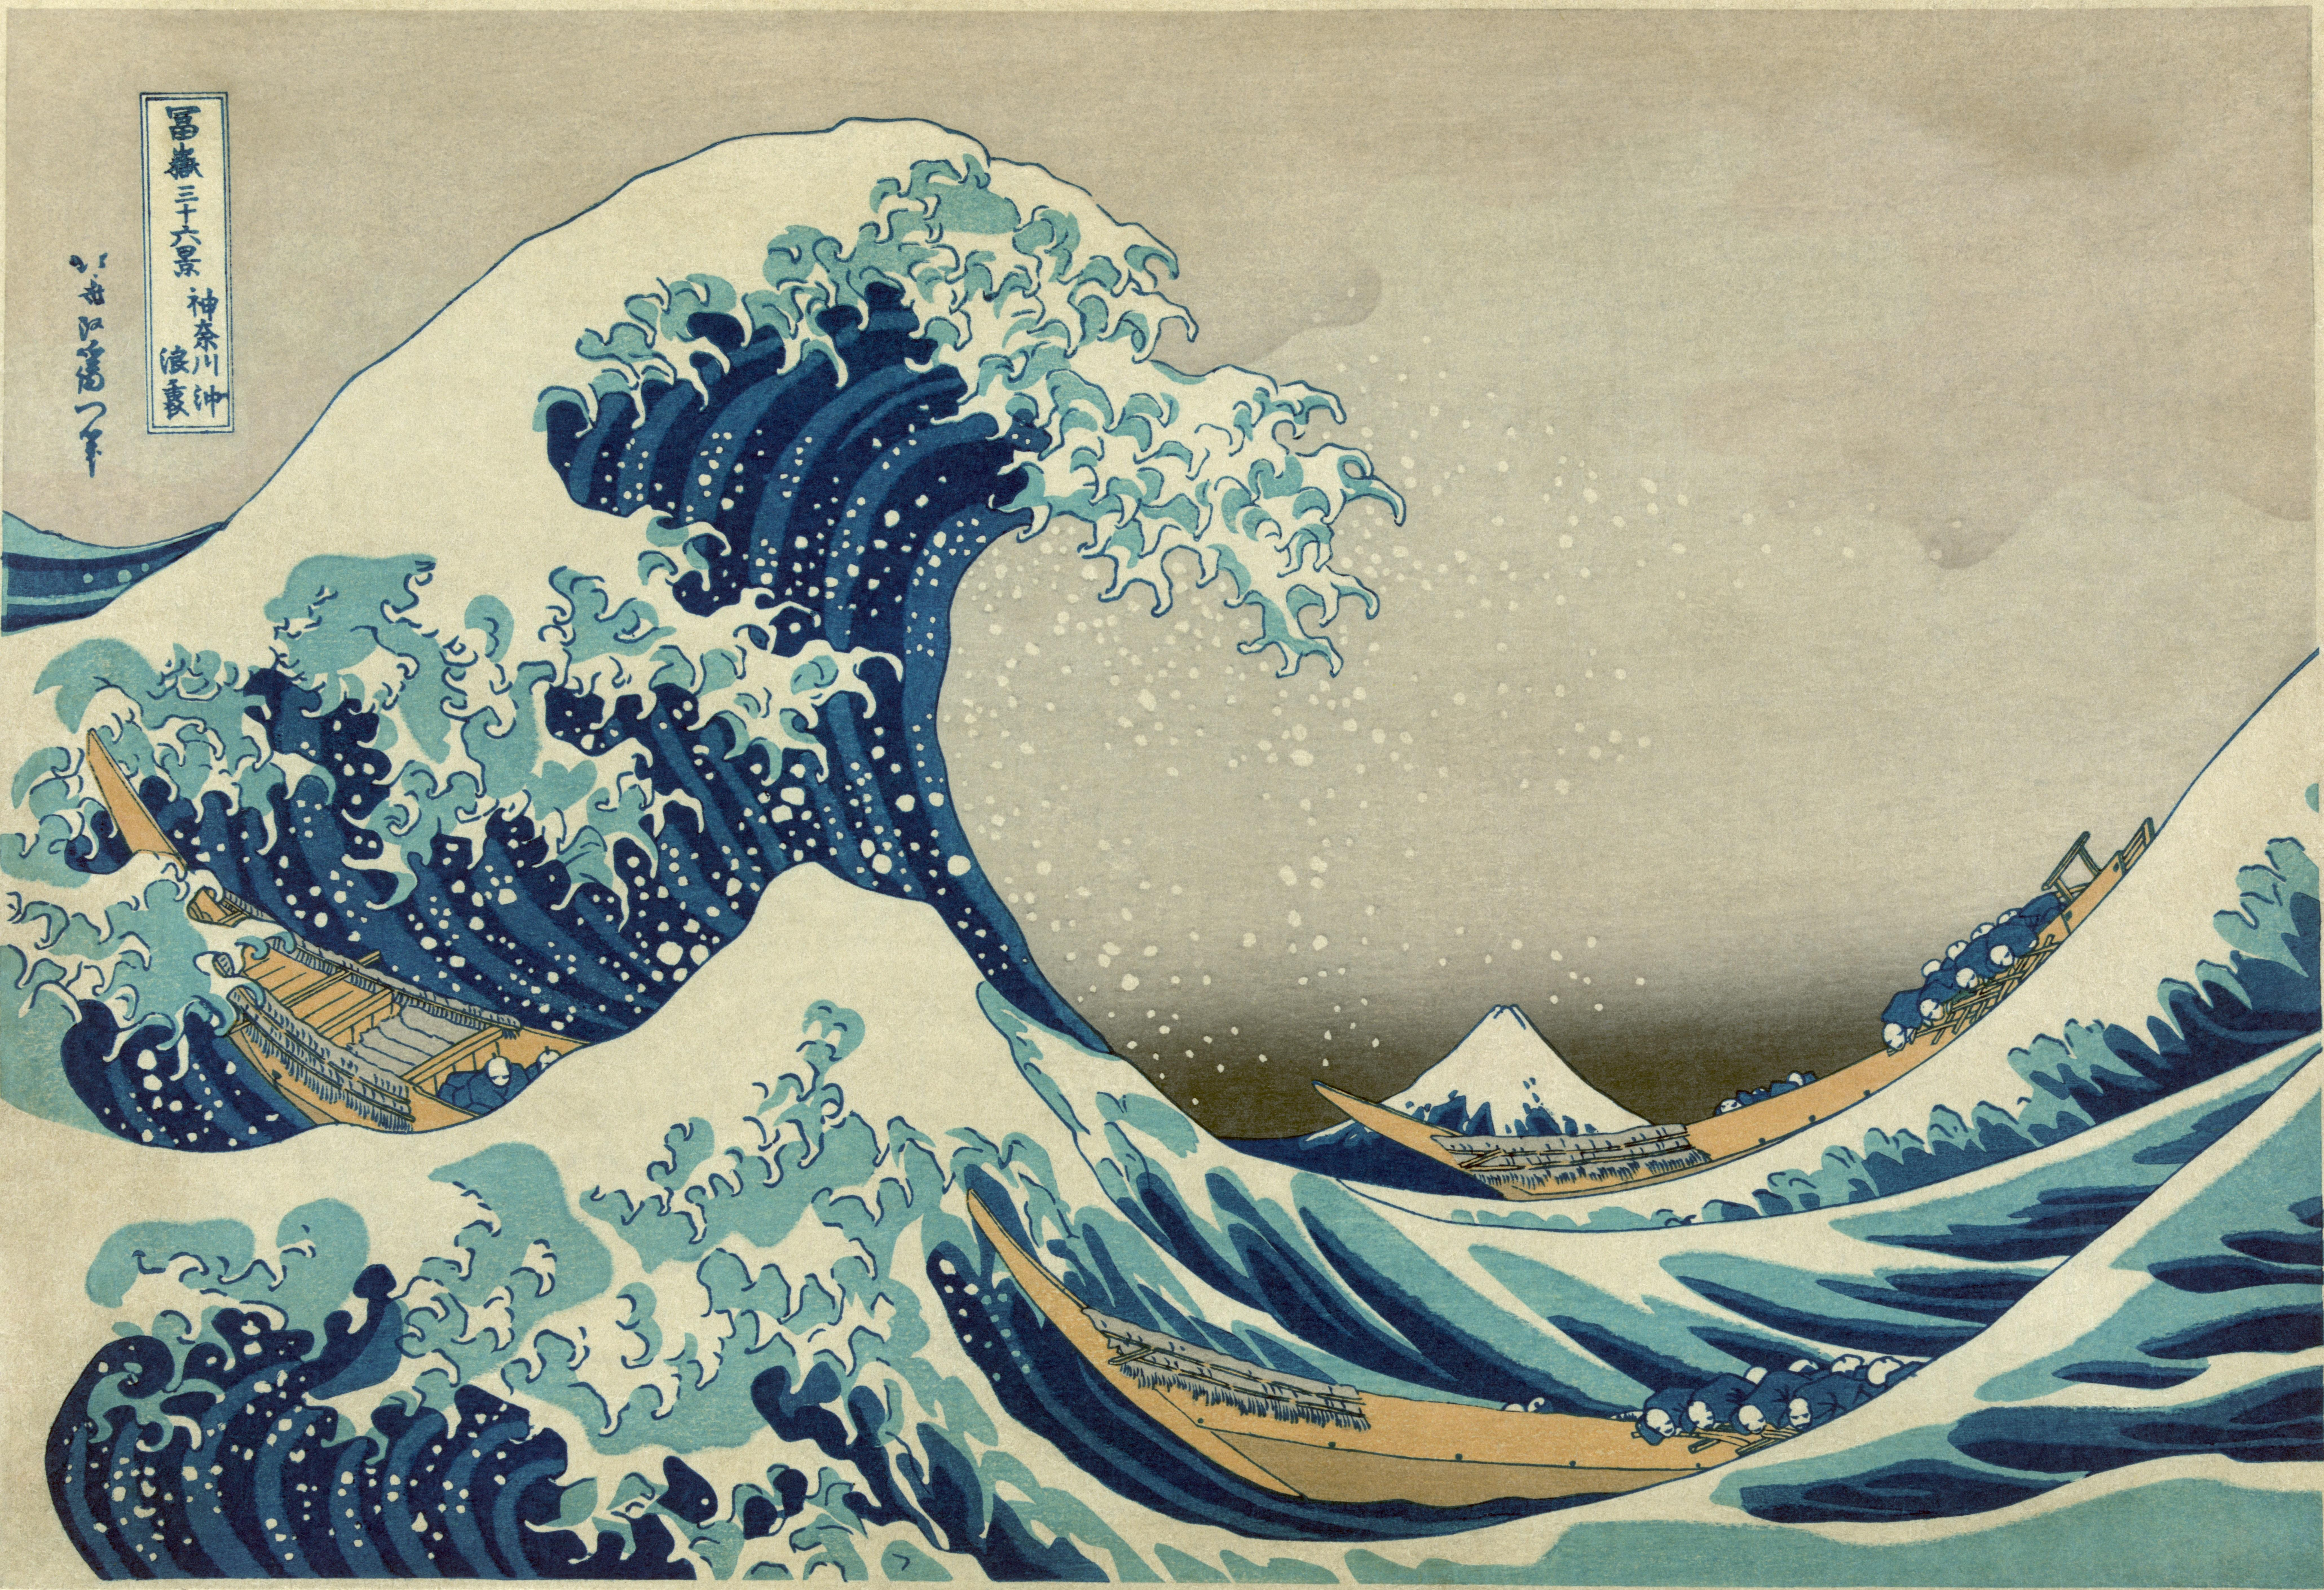
\includegraphics[width=\paperwidth]{images/kanagawa-wave.jpg}}
     };
   \end{tikzpicture}
 \end{center}

}


\clearpage

\restoregeometry
\nopagecolor


\begin{tcolorbox}
  {\color{BrickRed}\large\bfseries How to keep your book, code and data up to date}

  \paragraph{Book} The version number of the book is on the title page (or here: it is
  \BookVersionString). You can look for the latest version at \url{\BitLyBook}.
  When you run \texttt{l.update()}, it will tell you the most recent available version.

  \paragraph{Code} When you have a working \learninformatics\ environment, you can almost
  always update the code by typing \texttt{l.update()}. If there is a problem, you should
  manually replace the contents of \texttt{learninformatics.py} with
  \url{\BitLyCode}.

  \paragraph{Data} The data to support the judging of exercises lives in
  \texttt{DATA.txt}. This is always obtained and updated by typing \texttt{l.update()}.

  \bigskip
  Your exercises live in \texttt{main.py} and will never be affected by
  running an update.
\end{tcolorbox}

\paragraph{A special note for 0.2 users, 6 July 2021} Version 2.0 of the sofware and data
introduced a technology called YAML, which unfortunately does not work out-of-the-box with
replit.com. There might be a bit of manual updating required as I fix this issue.


\tableofcontents


\chaptermacro{Introduction}

The exercises in this document will enable you to progress from absolute informatics
novice to a level of confidence sufficient to tackle elementary problems on
ORAC\footnote{ORAC is an online judge found at orac2.info. Many other online judges exist,
such as dmoj.ca, hackerrank.com, and so on. ORAC has excellent problems, but its
input/output system is a pain, especially for beginners, and its entry-level problems,
while very easy, are still too hard for complete beginners.}, such as \emph{Cute Numbers},
\emph{Ladybugs}, and \emph{Drought}.

These exercises are self-contained and do not involve submitting code to a website. You
do, however, need to set up your Python coding environment a little. This up-front
inconvenience pays off very quickly, though, as you can:
\begin{itemize}
  \item Solve all problems in one file.
  \item Run your code interactively, or test it against known data, or have it judged
    against secret data, all with ease.
\end{itemize}

\emph{Describe the PLC Informatics system, or refer to Appendix A or whatever...}

The problems in Series 100 are generally original, though some inspiration naturally comes
from easy problems I've seen before. They have only a modicum of context, unlike later
informatics problems that require you to read paragraphs of text to discern exactly what
the problem is. Some problems will even give you some or all of the code required to solve
them! The aim is for you to experience a minimum of friction in the early part of your
learning.

\emph{Idea: mention here that we want to get right into it, but if you are reading this
with some interest but wondering what it's actually all about, please see Appendix A
``What is informatics anyway?''}

For ease of navigating the document, problems appear one per page. Please turn over and
begin.

\section*{Problems to develop}
\begin{itemize}
  \item Input \texttt{940 5 . + 30 . -5 . + 100 . + 12 . - 4} representing a starting
    value and a series of additions and subtractions. Output \texttt{940 . 970 . 965 .
    1065 . 1077 . 1073} representing the starting value, the intermediate values, and the
    answer. Story can be something like profits and losses each week, and wanting to see
    that the business is afloat. Perhaps if an intermediate value is negative, the output
    can include a warning alongside it.
  \item Sarah has taken up jogging. She starts at $D$ metres per day and increases her
    distance by $I$ metres each day. How many days until she is running 10 kilometres per
    day?
  \item Siobhan has taken up jogging. She starts at $D$ metres per day and increases her
    distance by $I$ metres each day until she reaches her limit of $M$ metres per day.
    Find the total distance she covers in $N$ days.
  \item Find the length of a Collatz chain starting at a given number.
  \item Find which starting number between $A$ and $B$ produces the longest Collatz chain.
  \item Four people (Albert, Betty, Charlie, Dolly) play several games of Scrabble. They
    know who won each game but have lost track of their overall tally. Input: $N$ lines of
    names. Output: \texttt{Albert: 48 . Betty: 37} etc.
  \item Cute numbers
\end{itemize}


% ---------------------------------------------------------------- Chapter 1: Basics

\setcounter{problemnumber}{100}

\chapter{Operating on a fixed set of numbers}

In these problems, you will read in just one number, or a list of numbers of a known size.
You will calculate something or somethings based on the input and write it to output.

The example problems and solutions shown here demonstrate how to read numbers (integers
and floats) from \IN\ and write results to \OUT. Note that when we write a float%
\footnote{In computing, decimal numbers are generally called ``floats'', short for
    ``floating point numbers'', because the location of the decimal point can float around
    (consider 104.32 and 1.0432, for instance).}
to \OUT, we must round it to the specified number of decimal places to ensure predictable
output.%
\footnote{If you use Python, or pretty much any programming language, to calculate
  $0.1+0.2$ then you will get a surprising result. It's not Python's fault; we have to live
  with the fact that computers, by default, don't handle decimal numbers particularly
well.}

The following lines of code demonstrate how to input and output integers and floats. 

\begin{pythoncode} 
  import learninformatics as l

  def example1(IN, OUT):
    a = int(IN.readline())
    b = float(IN.readline())

    print("a squared:", a*a, file=OUT)
    print("b squared:", b*b, file=OUT)
    print("b squared (2dp):", round(b*b,2), file=OUT)
\end{pythoncode}

You should enter this code, then run it, then type \pycode|l.run(example1)| in your shell.
It will wait while you enter two numbers (an integer and a float) and will then
immediately output the squares that the code promises.

The first two problems in this chapter are complete worked examples to show input and
output in some more context and to demonstrate some decision-making. After that, problems
will have fewer hints as you are expected to apply the skills learned in the earlier
problems.

\begin{quote}
  \color{blue}
  To assist in your learning, you should have a notebook where you write out your solution
  to each problem, along with notes on what you have learned. You will find that you refer
  to it often.
\end{quote}

When you solve actual numbered problems, you will write functions with names like
\pycode|ex101| (short for ``exercise 101''. You can then run the function interactively,
as you did with \pycode|example1|, but you can also do something even better: run it
against test data and judging data. These ideas were explained in the Introduction.

% ---------------------------------------------------------------- 101 Classify a triangle

\clearpage

\questionheader{\theproblemnumber\ Classify a triangle \workedexample}

\Question Read three integers representing sides of a triangle and
determine whether the triangle is equilateral, isosceles, or scalene.

\Sample

\minipagesthree{\sample{0.25}{17\\14\\13}{0.25}{scalene}}
               {\sample{0.25}{13\\13\\8}{0.25}{isosceles}}
               {\sample{0.25}{5\\5\\5}{0.25}{equilateral}}

\Solution

\begin{pythoncode} 
  def ex101(IN, OUT):
    a = int(IN.readline())
    b = int(IN.readline())
    c = int(IN.readline())

    if a == b and a == c:
      answer = 'equilateral'
    elif a == b or a == c or b == c:
      answer = 'isosceles'
    else:
      answer = 'scalene'

    print(answer, file=OUT)
\end{pythoncode}

\Explanation\ Lines 2--4 read the three lines in \IN\ into integer variables $a$, $b$ and
$c$. Lines 6--11 determine the answer, and Line 13 writes the answer to \OUT.

This program is very much about making decisions (\pycode|if|/\pycode|elif|/\pycode|else|)
with a small amount of data. Note the use of \pycode|and| and \pycode|or| in making the
decisions. \pycode|elif| is short for ``else if''.

Line 1 wraps this code up in a function called \pycode|ex101|, which is what the
\textbf{learninformatics} environment expects to find when you...well, see below.

\Running

The Introduction explained the features of the \textbf{learninformatics} environment. Now
we see them for ourselves.

After you have \emph{Run} your code in replit.com, try the following in the console.
\begin{itemize}
  \item \pycode|l.run(101)|, then use the keyboard to enter the values \texttt{15},
    \texttt{15} and \texttt{13}. The answer \texttt{isosceles} should immediately be
    displayed.
  \item \pycode|l.run(101, "15\n19\n20\n")|. This puts the data in directly, instead of
    waiting for you to type it. The answer \texttt{scalene} should immediately be
    displayed.
  \item \pycode|l.samples(101)|. This runs your code against the three samples shown
    above and checks that the correct output is produced. If the output is incorrect, or
    if an error occurs, a helpful report is printed so you can try to work out what went
    wrong.
  \item \pycode|l.judge(101)|. This runs your code against a greater variety of inputs and
    checks for the correct output. The inputs remain secret, the information printed if
    something goes wrong is quite basic. If your code passes all tests, a success token is
    printed as a reward.
\end{itemize}

Note that the name of the function containing your solution is important. If you call it
\pycode|training101| or \pycode|unicorn|, or anything other than \pycode|ex101|, then the
actions above will not work.

\begin{tcolorbox}
  As you proceed through the exercises, you will have many \texttt{def}s in your code, one
  for each exercise. This is excellent: a record of your work that you can look back on.
\end{tcolorbox}


% -------------------------------------------------------------- 102 Calculate a gradient

\clearpage

\questionheader{\theproblemnumber\ Calculate a gradient \workedexample}

\Question Read four floats representing points $(x_1,y_1)$ and
$(x_2,y_2)$ and find the \emph{gradient} of the interval $AB$, which is typically called
$m$ and is calculated as follows:
\[ m = \frac{\mathrm{rise}}{\mathrm{run}} = \frac{y_2 - y_1}{x_2 - x_1}.\]

Output the gradient, rounded to three decimal places.  If the gradient is undefined
(because the run is zero), output \texttt{undefined}.

\Sample

\minipagesthree{\sample{0.25}{5\\1\\10\\3.5}{0.25}{2.500}}
               {\sample{0.25}{-2.76\\-1.01\\3.14159\\-10.559}{0.25}{-1.693}}
               {\sample{0.25}{3.7\\9.5\\3.7\\17}{0.25}{undefined}}

\Explanation\ The answers given reflect the following calculations:

\vspace{-5mm}
\minipagesthree{\[\frac{3.5-1}{10-5} = 2.5\]}
               {\[\frac{-10.559 - (-1.01)}{3.14159 - (-2.76)} = -1.692594\ldots\]}
               {\[\frac{17 - 9.5}{3.7 - 3.7} = \frac{7.5}{0}\]}


\Solution

\begin{pythoncode} 
  def ex102(IN, OUT):
    x1 = float(IN.readline())
    y1 = float(IN.readline())
    x2 = float(IN.readline())
    y2 = float(IN.readline())

    rise = y2 - y1
    run  = x2 - x1

    if run == 0.0:
      answer = 'undefined'
    else:
      answer = rise / run

    print(round(answer,3), file=OUT)
\end{pythoncode}

\Explanation\ Lines 2--5 read the four floats from \IN\ and assign them to sensible
variable names. Lines 7--8 calculate the rise and run, which are important values in
determining the gradient. Lines 10--13 determine the answer, looking out for the undefined
case. Line 15 outputs the answer to \OUT, rounding it to three decimal places as required.

\Running\ The function is named \pycode|ex102|, so you can:
\begin{itemize}
  \item Run the code interactively with \pycode|l.run(102)|.
  \item Test the correctness of the code against some data with \pycode|l.samples(102)|
    and \pycode|l.judge(102)|.
\end{itemize}

\questionheader{\theproblemnumber\ Who is the tallest (1)? \stronghint}

\Question\ In the schoolyard you determine who is the tallest by standing back to back.
Among your online friends, though, the only way to find this out is to compare numbers.
There are four people in your group, and so when everyone has entered their height in
centimetres, all that remains is to pick the largest number out of the list.

Your program will read four numbers from \IN\ and write the largest number to \OUT.

\Sample

\sample{0.2}{147\\165\\171\\168}
       {0.2}{171}

\Scratch\ We've seen several examples now of how to read an integer from \IN. For this
problem, we need to do it four times.

\begin{pythoncode}
    a = int(IN.readline())
    b = int(IN.readline())
    c = int(IN.readline())
    d = int(IN.readline())
\end{pythoncode}

We now have all our data. All that remains is to decide which is the largest of $a$, $b$,
$c$ and $d$.

\begin{pythoncode}
    if a >= b and a >= c and a >= d:
        ...
\end{pythoncode}

If the condition above is true, then $a$ is the largest of the four, or at least the equal
largest. What do we do in this scenario?

\begin{pythoncode}
    if a >= b and a >= c and a >= d:
        answer = a
\end{pythoncode}

We store the value of $a$ in a new variable called \emph{answer}.

To the two lines of code provided above, you can add six more to make a complete
determination of the largest value among $a$, $b$, $c$ and $d$.

\Solution\ A complete solution looks like this, except for the six lines you need to add.

\begin{pythoncode}
    def ex103(IN, OUT):
        a = int(IN.readline())
        b = int(IN.readline())
        c = int(IN.readline())
        d = int(IN.readline())

        if a >= b and a >= c and a >= d:
            answer = a
        #
        # ...six more lines...
        #

        print(answer, file=OUT)
\end{pythoncode}

If you're really stuck, you can look at the answers provided.

\Afterword\ The detailed assistance provided in this example was painstaking, so this will
be gradually decreased over the next few problems.

As you coded this problem, you might have had two questions.
\begin{itemize}
    \item Is this \emph{really} the best way to find the largest of four numbers?
    \item What if there were 400 numbers instead of four?
\end{itemize}

These questions will be addressed in \emph{Who is the tallest? (2)} and \emph{Who is the
tallest? (3)} respectively.


\questionheader{\theproblemnumber\ The cheapest TV}

\Question\ You walk the aisles of Bing Lee, looking for a new TV. You narrow it down to
five choices and decide to go with the cheapest. How much will you pay?

Your program will read five integers (representing prices in dollars) from \IN\ and write
the smallest number to \OUT.

\Sample

\sample{0.2}{499\\565\\325\\400\\717}
       {0.2}{325}

\Scratch\ If you have learned the lessons of the previous exercise well, you will complete
this one in no time. The running instructions are the same as before except the problem
name is \problemtagtt.

\Afterword\ Run your code as before. Brief instructions are included here for the last time:
\begin{itemize}
    \item \code{p.run(\problemtag)} to run it interactively using keyboard and screen.
    \item \code{p.test('\problemtag', \problemtag)} to run it against some test data and
      get detailed information if there is an error.
    \item \code{p.judge('\problemtag', \problemtag)} to run it against some judging data
      and get a token if you are successful.
\end{itemize}


\questionheader{\theproblemnumber\ Shopping (1)}

\Question\ You've just returned from the shops with the items you were asked to get. Your
dad asked ``How much was it?'', but you don't remember! You have to work it out quickly.
You bought exactly three \emph{kinds} of items, but different \emph{quantities} of each.

\Input

The input contains six lines: quantity 1, price 1, quantity 2, price 2, quantity 3, price
3. The quantities are integers in the range 1--10 and the prices are positive floats less
than 100 (representing \$100).

\Output\ The output is a single float containing the total price, and it must be rounded
to two decimal places.

\Sample

\sample{0.2}{6\\2.50\\8\\1.75\\3\\87.88}
       {0.2}{292.64}

\Explanation The output represents \$292.64, which is $6(\$2.50) + 8(\$1.75) + 3(\$87.88)$.

\Scratch\ You already know how to read an integer from \IN. See \futurereference{Appendix
...} for advice on reading and writing floats, especially outputing them rounded to two
decimal places.



\questionheader{\theproblemnumber\ Jogging (1)}

\Question\ Sarah is about to take up jogging. She will start jogging $D$ metres per day
and increase her daily distance by $I$ metres each day. When she reaches her target of $T$
metres per day, she will stop the daily increase and just keep a consistent jogging
pattern.

How many days after she starts will she reach her target?

\Input

The input contains three lines, all of which are values in metres:
\begin{itemize}
  \item $D$, the distance at which she starts jogging;
  \item $I$, the amount by which she increases her jog each day;
  \item $T$, her target daily jog, after which she doesn't increase it any further.
\end{itemize}

All values are integers, and you are guaranteed that $D < D+I < T$, that is, she will have
to apply at least two increases before reaching her target.

\Output\ You will write a single integer to \OUT, that being the number of days after
starting that she reaches her target.

\Sample

\minipagestwo{%
  \sample{0.4}{100\\50\\300}
         {0.4}{4} }{%
  \sample{0.4}{700\\20\\750}
         {0.4}{3} }


\Explanation In the first sample, her running pattern over the days goes like this:
\begin{center}
  \begin{tabular}{cc}
    Day & Distance (m) \\
    1   & 100\\
    2   & 150\\
    3   & 200\\
    4   & 250\\
    5   & 300
  \end{tabular}
\end{center}

She reaches her target on day 5, which is four days after she starts jogging, so the
answer is \texttt{4}.

In the second sample, her running pattern \emph{would} proceed 700, 720, 740, 760, but
\SI{760}{\m} actually exceeds her target of \SI{750}{\m}, so she would in fact run
\SI{750}{\m} on the fourth and subsequent days. In any case, she reached/exceeded her
target on day 4, which is three days after she started, so the answer is \texttt{3}.

\Scratch\ It is intended that you use simple mathematics to work this out. As a very large
hint, consider the expression $(300 - 100)/50$ in the first sample. As another hint, be
aware of the difference between \pycode|/| and \pycode|//| in Python. Finally, although
it's not strictly necessary, you might benefit from searching for examples of
\pycode|math.floor| and \pycode|math.ceil|.


\questionheader{\theproblemnumber\ Who is the tallest (2)?}

\emph{This question takes another look at \futurereference{Problem 101}.}

\Question\ In the schoolyard you determine who is the tallest by standing back to back.
Among your online friends, though, the only way to find this out is to compare numbers.
There are four people in your group, and so when everyone has entered their height in
centimetres, all that remains is to pick the largest number out of the list.

Your program will read four numbers from \IN\ and write the largest number to \OUT.

\Sample

\sample{0.2}{147\\165\\171\\168}{0.2}{171}

\Scratch\ Just like the earlier problem (\futurereference{Tallest person (1)}), we need to
read four integers from \IN. But this time, instead of making a lot of comparisons between
$a$, $b$, $c$ and $d$, we will use Python's built-in \code{max} function.

If you try the following Python expressions in your shell...

\begin{pythoncode}
    max(5, 1, 2, 9)
    max(7, 2, 5, 11, 6)
    max(-51, 73, 33, -1, 0, 12)
\end{pythoncode}

...then you will learn with some relief that Python has pretty much solved the ``Who is
the tallest?'' problem for us.

\Solution\ Make a new function \emph{in the same file}:

\begin{pythoncode}
    def train102(IN, OUT):
        a = int(IN.readline())
        b = int(IN.readline())
        c = int(IN.readline())
        d = int(IN.readline())

        answer = max(a, b, c, d)

        print(answer, file=OUT)
\end{pythoncode}

Use the tag \problemtagtt\ when you test and judge your code.

\Afterword\ The \pycode|max()| function can take any number of arguments, or it can find
the maximum of a (potentially very long) list. These are details for later. But here are
two teasers that you can run in the shell and think about.

\begin{pythoncode} 
  max(n*n for n in [-6, -4, -1, 0, 3])
  max(len(x) for x in ["Emma", "Caitlin", "Tim"])
\end{pythoncode}



\questionheader{\theproblemnumber\ A fair wage (1)}

\Question\ There are six employees in your company all doing roughly the same kind of
work. Some have worked for you for a longer time, or are generally more productive, so you
pay them a bit more. But once a year you take a look to see if the overall distribution of
wages seems to be fair.

The first thing you look for is the \emph{range} of wages: the highest minus the lowest.
You have a rule that the range should be less than 10\% of the highest wage.

\Input\ From \IN\ you will read six floats, each representing a weekly wage.

\Output\ To \OUT\ you will write three values:
\begin{itemize}
  \item The range, rounded to two decimal places
  \item The highest wage, rounded to two decimal places
  \item \texttt{yes} or \texttt{no} according to whether your wages are fair
\end{itemize}

\Sample

\minipagestwo{\sample{0.4}{535.00\\517.50\\580.00\\575.89\\553.60\\521.45}
                     {0.4}{62.5\\580.0\\no}}
             {\sample{0.4}{535.00\\517.50\\570.00\\570.00\\553.60\\521.45}
                     {0.4}{52.5\\570.0\\yes}}

\Explanation\ In the first sample, the range is about 10.78\% of the maximum wage, thus
the wages are not fair. In the second sample, the range is about 9.21\% of the maximum
wage, thus the wages are fair.

\Scratch\ After completing \emph{Who is the tallest? (2)}, you should be comfortable
reading six numbers and finding their maximum. To find the minimum, just use \pycode/min/
instead of \pycode/max/.

See the first code listing in Chapter 1 if you need a refresher on outputing floats
rounded to two decimal places.



% ---------------------------------------------------------------- Chapter 2: Loops (1)

\setcounter{problemnumber}{200}

\chapter{Looping through data}

In the problems you've encountered so far, you would:
\begin{itemize}
  \item read a fixed number of items from \IN;
  \item perform some calculation on those items;
  \item write a result to \OUT.
\end{itemize}

I'm sure you understand, though, that most problems don't come with a fixed number of
items of input, and sooner or later you will need to write code that can handle input of
any size. Well, that time is now.

\questionheader{\theproblemnumber\ Shopping (2)}

\Question\ You are in the middle of a sizeable shopping trip and realise you may not have
enough money to pay for everything you have put in your trolley. Quickly, you write a
program that takes in the quantities and prices of all the items you intend to purchase
and reports the total price.

\Input

The first line of input is $N$, which is the number of quantity-item pairs. Following this
are $2N$ lines, each pair of which contains the quantity and the price. The example will
make this clear.

\begin{itemize}
  \item $0 < N < 10\,000$.
  \item Each quantity $Q_i$ is an integer that satisfies $0 < Q_i < 1000$.
  \item Each price $P_i$ is a float that satisfies $0.00 < P_i < 1000.00$.
\end{itemize}

\Output\ The output is a single float containing the total price, and it must be rounded
to two decimal places.

\Sample

\sample{0.2}{5\\4\\2.99\\1\\3.15\\2\\14.95\\19\\0.14\\7\\7.10}
       {0.2}{97.37}

\Explanation The output represents \$97.37, which is $4(\$2.99) + 1(\$3.15) + 2(\$14.95)
+ 19(\$0.14) + 7(\$7.10)$.



\questionheader{Sum of squares}

\Question\ Given a scatterplot, there are a few ways to mathematically determine an
objective line of best fit. One way is to find the line that has the least sum-of-squares
when considering the distance from each point to the line.%
\footnote{See https://www.mathsisfun.com/data/least-squares-regression.html for a nice
overview of this.}

In preparation for writing a program to find the line of best fit, then, you start by
finding the sum of squares of $N$ floating-point numbers.

\Input\ The first line contains the positive integer $N$, the number of data points for
you to consider. The next $N$ lines each contain a float, $D_i$.

\Output\ A single float, rounded to two decimal places, that represents the sum of squares
\[
  (D_1)^2 + (D_2)^2 + (D_3)^2 + \dots + (D_N)^2.
\]

\Sample

\sample{0.2}{5\\6.2\\-1.7\\4.29\\3.815\\-2}
       {0.2}{73.88}

\Scratch\ The important variable here, as with the previous problem, is \emph{total}.
Initialise it to zero and add the square of each input number.


\questionheader{Check the invite list \workedexample}

\Question\ Iliana is planning a party. Like, the best party e-vah! She already has a draft
list of who she wants to invite, but now her friend Alona mentions a new name. Or is it
new!? We'll have to check the invite list to find out.

\Input\ From \IN\ you will read:
\begin{itemize}
  \item a name $Q$, the person whose invite-status is being questioned;
  \item a positive integer $N$, the number of people on the draft invite list;
  \item $N$ names $I_1$ to $I_N$, representing people who are on the draft invite list.
\end{itemize}

\Output\ A single line to say whether the name $Q$ appears on the draft invite list, and
if so, where. The samples make this clear.

\Sample

{\small
\minipagestwo{%
  \sample{0.2}{Kevin\\5\\Jenny\\Tonya\\Sandy\\Erin\\Mike}
         {0.6}{Kevin is not yet invited}
}{%
  \sample{0.2}{Kevin\\6\\Jenny\\Tonya\\Sandy\\Kevin\\Erin\\Mike}
         {0.6}{Kevin is \#4 on the list}
}
}

\Explanation\ In the first sample, we are determining whether Kevin appears in the list
Jenny, Tonya, Sandy, Erin and Mike. Kevin is \emph{not} among those names, hence the
output \texttt{Kevin is not yet invited}. In the second sample, Kevin \emph{is} among the
names and appears in position number 4, hence the output \texttt{Kevin is \#4 on the
list}.

\Scratch\ This exercise brings you two new skills:
\begin{itemize}
  \item reading and working with strings; and
  \item keeping track of where we are in the list.
\end{itemize}

Remember also that you can \pycode|break| out of a loop. In the second sample, once you
find Kevin in position 4 you know what output is required, so there's no need to continue
reading names.

\textbf{Reading strings} from \IN\ is very straightforward. Here's the summary:
\begin{pythoncode}
  name = IN.readline().strip()
\end{pythoncode}

There are two things to notice about this use of \pycode|readline()| compared to what
we usually do.
\begin{enumerate}
  \item There is no \pycode|int(...)| or \pycode|float(...)| because we are \emph{not}
    dealing with numerical data.
  \item We append \pycode|.strip()| to remove the newline character at the end.
\end{enumerate}

To explain the second item further, \pycode|readline()| reads a \emph{line} of input,
exactly as it says. And a line is terminated by a \emph{newline} character, which is what
gets collected when you hit the Enter or Return key. So you might like to think that
reading the second line of the sample input(s) gives you \pycode|'Kevin'|, but
unfortunately it does not; you get \pycode|'Kevin\n'|. Calling \pycode|.strip()| on this
string removes any whitespace from the left or right, giving us the \pycode|'Kevin'| that
we want.

Here is a simple example you can try. Run it with \pycode|l.run(newline_example)| and type
two strings as input (e.g. \texttt{Hello} and \texttt{Goodbye}).
\begin{pythoncode}
  def newline_example(IN, OUT):
    a = IN.readline()
    b = IN.readline().strip()
    print('a: {repr(a)}  b: {repr(b)}', file=OUT)
\end{pythoncode}

The special function \pycode|repr|%
\footnote{See docs.python.org/3/library/functions.html}
gives you a programmer's view of what an object is, thus it explicitly \emph{shows} you
the newline character instead of \emph{printing} it.

\textbf{Working with strings} for this problem means asking whether two strings are the
same. This is no different from asking whether two integers are the same. You can try the
following in the console:
\begin{pythoncode}
  'Kevin' == 'Kevin'        # True
  'Kevin' == 'Andy'         # False
  'Kevin' > 'Andy'          # True (alphabetical order)
\end{pythoncode}

\textbf{Keeping track of where we are} is also easy enough, but to ensure understanding we
need to look at a few ways of doing it. To develop this, we assume that our code will look
something like this
\begin{pythoncode}
  for i in range(N):
    name = IN.readline().strip()
    # ...
\end{pythoncode}
and build around it.

Before we look at any code, consider the trace table we are trying to achieve, using the
second sample as input.

\begin{center}
  \begin{tabular}{cl}
    \toprule
    position & name \\
    \midrule
    1 & Jenny \\
    2 & Tonya \\
    3 & Sandy \\
    4 & Kevin \\
    \bottomrule
  \end{tabular}
\end{center}
\medskip

The fifth and sixth names are not shown as we would stop reading when we find
Kevin, and we would have the information we need to report that he is \#4 in the list.

The first approach is to have a variable called \pycode|position| that we initialise to 1
and update each time we go through the loop.
\begin{pythoncode}
  position = 1
  for i in range(N):
    name = IN.readline().strip()
    # ...
    position = position + 1
\end{pythoncode}

This could be written with a \pycode|while| loop instead of a \pycode|for| loop, but it's
not an improvement.

\begin{pythoncode}
  position = 1
  i = 0
  while i < N:
    name = IN.readline().strip()
    # ...
    position = position + 1
    i = i + 1
\end{pythoncode}

However, it occurs to us that we might not need \emph{both} \pycode|position| and
\pycode|i|. The purpose of \pycode|i| is to run the loop the correct number of times; this
duty could be performed by \pycode|position| instead.

\begin{pythoncode}
  position = 1
  while position <= N:
    name = IN.readline().strip()
    # ...
    position = position + 1
\end{pythoncode}

That's better. And now that we have a conceptually clean approach, we can translate it
back into a \pycode|for| loop.

\begin{pythoncode}
  for position in range(1, N+1):
    name = IN.readline().strip()
    # ...
\end{pythoncode}

In that final piece of code, we don't need to assign or update \pycode|position| manually;
the \pycode|for| loop takes care of it for us. We just need to specify what we want the
range to be.

\textbf{We solve the problem} by the following steps.
\begin{enumerate}
  \item Read $N$ and $Q$ and set them to variables \pycode|N| and \pycode|target_name|.
  \item Set a variable \pycode|found| to \pycode|False|. We need to know whether we found
    the name or not.
  \item Use \pycode|for position in range(1, N+1):| to loop $N$ times while keeping track
    of the position $(1,2,3,\dots,N)$.
  \item Each time through the loop, we read a name (and strip the newline). If it's equal
    to \pycode|target_name|, set \pycode|found| to \pycode|True| and break out of the
    loop. If it's not equal to \pycode|target_name|, there's nothing special we need to
    do, just let the loop run again.
  \item When the loop finishes (either by \pycode|break| or by running out of items to
    read), we need to print the answer, which depends on whether the target name was
    \pycode|found| or not.
\end{enumerate}

\Solution

\begin{pythoncode}
  N = int(IN.readline())
  target_name = IN.readline().strip()
  found = False

  for position in range(1, N+1):
    name = IN.readline().strip()
    if name == target_name():
      found = True
      break

  if found:
    print(f'{target_name} is #{position} on the list', file=OUT)
  else:
    print(f'{target_name} is not yet invited', file=OUT)
\end{pythoncode}

\bigskip
Here are trace tables for the two examples.
\medskip

\minipagestwo{
  \begin{center}
    \begin{tabular}{clc}
      \toprule
      position & name & found \\
      \midrule
      1 & Jenny & False\\
      2 & Tonya & False\\
      3 & Sandy & False\\
      4 & Erin  & False\\
      5 & Mike  & False\\
      \bottomrule
    \end{tabular}
  \end{center}
}{
  \begin{center}
    \begin{tabular}{clc}
      \toprule
      position & name & found \\
      \midrule
      1 & Jenny & False\\
      2 & Tonya & False\\
      3 & Sandy & False\\
      4 & Kevin & True\\
      \bottomrule
    \end{tabular}
  \end{center}
}


\questionheader{Scrabble tally}

\Question\ Four friends---Albert, Betty, Charlie and Dotty---have played a lot of Scrabble
games over the years. The competition has been pretty close, but they've all kind of
forgotten who has won how many games. Luckily, when moving house recently, Dotty unearthed
a long list of the winners of all their games! By processing this list, you will be able
to give them a full tally.

\Input\ The first line of \IN\ contains $N$, the number of winners listed. Following this
are $N$ lines, each of which contains the name \texttt{Albert}, \texttt{Betty},
\texttt{Charlie} or \texttt{Dotty}, representing the winner of one game.

\Output\ \OUT\ contains four lines, reporting a tally as seen in the sample.

\Sample

\sample{0.25}{10\\Dotty\\Albert\\Albert\\Charlie\\Dotty\\Albert\\Dotty\\Dotty\\Dotty\\Charlie}
       {0.2}{Albert: 3\\Betty: 0\\Charlie: 2\\Dotty: 5}

\Scratch\ In this problem, you are reading \emph{strings} for the first time. ``String''
is the computer-science word for textual data, presumably because the characters are
``strung'' together. To read a string, we could simply call \pycode|IN.readline()|, with
no \pycode|int(...)| or \pycode|float(...)| wrapper because we certainly do not want
Python to attempt to convert our names to numbers.

There's a sting quite literally in the tail, though, because when we read a line of data
from \IN, the resulting string has a newline character at the end, and we don't really
want that.


\questionheader{Buried treasure}

\Question\ Your Pacific Islands cruise has pulled up near a small but enticing island and
you and hundreds of other tourists have gone ashore for a day of sun, swimming and
scoffing ``authentic'' local foods and drinks. Tiring of the tourist traps, you wander off
the beaten path into the bush, where in addition to some peace and quiet, you find a scrap
of paper that happens to contain a map of the island and a promise of buried treasure! No
doubt it is fake, but with not much else to do until the dinghy returns you to the
floating RSL at 3.30\,pm, you might as well take a closer look.

The map divides the island neatly into square units. It has a list of N/S/E/W directions
listed, and you interpret that as taking a one-unit step in the specified direction.
So if you started at location $(4,6)$ and took steps ``N'', ``N'' and ``W'', you would end
up at location $(3,8)$.

Sometimes the direction given is the full word (North, South, East, West). Sometimes it is
the abbreviation (N, S, E, W). Capitalisation is always consistent. If you encounter any
instruction other than the eight specified then it is invalid.

So the question is: given a starting location and a list of directions, where might the
treasure be buried?

\Input From \IN\ you will your location and a list of directions.

\begin{itemize}
  \item The first line contains $X$, the $x$-value of your location.
  \item The second line contains $Y$, the $y$-value of your location.
  \item The third line contains $N$, the number of directions in the list.
  \item The next $N$ lines contain $D_i$, a direction that is either North, South, East,
    West, N, S, E, W or else it is an invalid direction.
\end{itemize}

Note that $X$ and $Y$ are integers such that $-1000 \le X,Y \le 1000$ and $N$ is an integer
such that $1 \le N \le 1000$.

\Output\ If all the directions are valid, you will output a single line $X'\ Y'$, being
your location after folloing the directions.

If you encounter an invalid direction, you will output the single line \texttt{Invalid
directions}.

\Sample

\minipagestwo{
  \sample{0.22}{8\\-7\\6\\N\\North\\W\\N\\East\\E\\S}
         {0.45}{9 -4}
}{
  \sample{0.22}{8\\-7\\6\\N\\North\\Go right\\N\\East\\E\\S}
         {0.47}{Invalid directions}
}

\Explanation\ In the first sample, the starting position is $(8,-7)$ and the sequence
$[N,N,W,N,\allowbreak E,E,S]$ results in a final position of $(9,-5)$. In the second
sample, the instruction \texttt{Go right} is invalid.

\Scratch\ You might like to run through the first sample on paper, completing a trace
table with columns $i$, $dir$, $X$, and $Y$.


\questionheader{Area calculator}

\Question\ As you pore over your Maths homework, you tire of the seemingly endless and
pointless area calculations you have to do. All the circles, semicircles, rectangles,
squares, parallelograms and triangles demand so much attention, and you only have so much
to give. But if you write a program to do the calculations for you, you'll get this
wretched work done and have time for a camomile tea while watching \emph{Rick \& Morty}
before bed.

\Input

The input contains any number of lines, which represent the shape names and the values
required to calculate them. For circles and semicircles you get one value: the radius. For
rectangles, parallelograms and triangles, you get base and (perpendicular) height. For
squares, you get the length of one side. The last line of input is simply \texttt{stop}.

Your input will contain ten area calculations or fewer.

\Output\ The output contains several lines, each of which is the result of an area
calculation, which must be a float rounded to three decimal places.

\Sample

\sample{0.25}{circle\\4.6\\triangle\\12\\5\\parallelogram\\19\\4.5\\
             square\\19\\rectangle\\7.2\\3.6\\stop}
       {0.2}{66.476\\30.0\\85.5\\361.0\\25.92}

\Scratch\ This problem differs from the earlier ones in two ways:
\begin{enumerate}
  \item We are \emph{not} told at the beginning how many lines there will be.
  \item Depending on the shape, we may need to read one line or two.
\end{enumerate}

Therefore, you deserve some help with this problem.

To solve \#1, we want to loop \emph{endlessly} and break out of the loop when we read
\texttt{stop}. This can be done with the following code structure:
\begin{pythoncode}
  while True:
    # ...
    if (condition):
      break
    # ...
\end{pythoncode}

The \pycode|while True| part creates the endless loop, and the \pycode|break| statement
gets out of it. Naturally, the \emph{condition} for us to break out is having read the
word \texttt{stop}.

Solving \#2 is not difficult and you probably don't need help with it, but just in case,
there is a hint on the next page.

\clearpage

\Hint

Here is the structure of the code, excluding the function header.

\begin{pythoncode}
  while True:
    shape = IN.readline().strip()
    if shape == 'stop':
      break
    elif shape == 'circle':
      radius = float(IN.readline())
      area   = 3.141592654 * radius * radius
      print(round(area,3), file=OUT)
    elif shape == 'rectangle':
      base   = float(IN.readline())
      height = float(IN.readline())
      # ...
    # etc.
\end{pythoncode}



\questionheader{Drought}

\Question\ \grey{(Sourced from ORAC)}\quad Years of drought have hit rural Australia hard.
With catchment levels at an all time low, you decide to purchase a rainwater tank. Soon
the winter rains arrive, and the tank slowly begins to fill.

You begin to wonder just when your tank will be entirely full. A friend
in the weather bureau has kindly lent you rainfall predictions for the next few days.
Given these predictions, and the size of your rainwater tank, write a program to determine
how many days your tank takes to fill.

\Input\ The first two lines of the input file will contain the values $N$ and $C$, where
$N$ is the number of days the weather predictions last, and $C$ is the capacity of your
rainwater tank in litres.  You are guaranteed that $1 \le N \le 1000$, and that $C$ is a
positive integer no greater than the total amount of rain that falls over the $N$ days.

The remaining $N$ lines of input will describe the rainfall levels for each day in order.
Each line will contain a single integer between 0 and 1\,000\,000: the amount of rain (in
litres) that will fall over your rainwater tank that day.

\Output\ Your output should consist of a single integer: the number of days until your
rainwater tank fills.

\Sample

\minipagestwo{%
  \sample{0.4}{6\\10\\2\\3\\3\\2\\2\\4}
         {0.4}{4} }{%
  \sample{0.4}{6\\11\\2\\3\\3\\2\\2\\4}
         {0.4}{5} }


\Explanation\ In both examples, the total rainfall changes as follows:

\begin{center}
\begin{tabular}{cc}
  \textbf{Day} & \textbf{Running total (L)} \\[3pt]
  1 & 2 \\[1pt]
  2 & 5 \\[1pt]
  3 & 8 \\[1pt]
  4 & 10 \\[1pt]
  5 & 12 \\[1pt]
  6 & 16 \\[1pt]
\end{tabular}
\end{center}
\vspace{12pt}

Hence a 10-litre water tank is full after 4 days and an 11-litre water tank is full after
5 days.

\Scratch\ If you intialise a variable to track the running total to zero at the beginning
and keep it updated as you read in the data, you should be able to solve this.

Good to know: you can \pycode|break| out of a \pycode|for| loop just like you can a
\pycode|while| loop.


\questionheader{Cute numbers}

\Question\ \grey{(Sourced from ORAC)}\quad For you, numbers have personalities. The number
4 is elegant, 18 is strong and 42 is enigmatic.  And, of course, any number ending in 0 is
cute.  The more zeroes at the end of a number, the cuter that number is. Therefore $70$,
$36\,640$ and $1\,800\,090$ are only a little bit cute (ending in just one zero), whereas
400 and $99\,200$ are very cute (ending in two zeroes) and $30\,000$ is really really cute
(ending in four zeros).

Your task is to read in a number $N$ and determine how many zeros are at the end of that
number, so you can tell just how cute the number is.

\Input\ The first line of input will consist of the single integer $d$, telling you how
many digits are in the number $N$. You are guaranteed that $1 \le d \le 100\,000$.

Following this will be $d$ additional lines, each containing a single digit (0, 1, 2, 3,
4, 5, 6, 7, 8 or 9). These will be the digits of $N$, written from left to right. You are
guaranteed that the first digit of $N$ will not be zero.

\Output\ You must write a single integer as output, representing the number of zeroes at
the end of $N$.

\Sample

\minipagestwo{%
  \sample{0.4}{5\\9\\9\\2\\0\\0}
         {0.4}{2} }{%
  \sample{0.4}{7\\1\\9\\0\\0\\0\\9\\0}
         {0.4}{1} }


\Explanation The first example describes $N = 99\,200$, which ends in two zeros. The second
example describes $N = 1\,800\,090$, which contains many zeroes within but has only one zero
at the end.



\questionheader{Even numbers for photos! (1) \stronghint}

\Question\ Some cultures have a strong preference that when a photograph of a group of
people is taken, that the group comprise an \emph{even} number of people. You, as a
wedding photographer who is about to work at a wedding that is steeped in one such
culture, have been given a list of groups who will be photographed, and you need to
scrutinise it to see if there are any, um, \emph{odd} problems that need to be fixed.

The list just contains the \emph{number} of people in each planned photo. You decide to
analyse it as follows: highlight the \emph{chains} of odd numbers so that you might engage
in some creative rearranging. For instance, the list might read: \[
  \mathbf{7}
  \quad 8 \quad 10 \quad 8
  \quad \mathbf{11} \quad \mathbf{13} \quad \mathbf{11} \quad \mathbf{19}
  \quad 4
  \quad \mathbf{9} \quad \mathbf{15}
  \quad 6 \quad 8
\]

In this list, you are interested in the bolded chains, which have lengths 1, 4 and 2,
respectively. You are also interested in:
\begin{itemize}
  \item the total number of such groups (in this case, 7); and
  \item the total number of people involved in these photos (in this case, 91).
\end{itemize}

Knowing these things won't solve all your problems, but it's a start.

\Input\ The first line is a positive integer $N$, which is the number of data points to
follow. The next $N$ lines each contain a positive integer $P_i$, each of which is the
number of people planned to be in a photograph.

\Output\ You will output the \emph{length of each chain} of odd-numbered photographs.
After this, leave a blank line, and output the number of photos containing an odd number
of people, and the total number of people in these photos, on one line as shown in the
samples.

\Sample

\minipagesthree{
  \sample{0.3}{13\\7\\8\\10\\8\\11\\13\\11\\19\\4\\9\\15\\6\\8}
         {0.3}{1\\4\\2\\\ \\7:91}
}{
  \sample{0.3}{6\\5\\3\\4\\8\\6\\3}
         {0.3}{2\\1\\\ \\3:14}
}{
  \sample{0.3}{7\\4\\6\\4\\2\\6\\4\\6}
         {0.3}{\ \\0:0}
}

\Explanation\ The first sample represents the example given in the question. The second
sample has odd chains $[5,3]$ and $[3]$, hence the output \texttt{2} and \texttt{1}. The
summary for the second sample is three groups totalling 14 people, hence \texttt{3:14}.
The third sample has no groups with an odd number of people, so there are no chains to
report. There is still a blank line before the summary \texttt{0:0}, though.

\Scratch\ Try creating and completing a trace table for the first sample before
continuing. A hint is given over the page.

\clearpage % ------------------------------------------------------------------ new page
\questionheadercontinued{Even numbers for photos! (1)}

We assume the code structure shown below.
\begin{pythoncode}
  N = int(IN.readline())
  # other initialisations...

  for i in range(N):
    # ...
\end{pythoncode}

What are we tracking in this question? We want the \emph{number of groups} and the
\emph{number of people}, which suggests variables \pycode|ngroups| and \pycode|npeople|.

Here is a trace table that you could try to complete.

\begin{inlinetable}
  \sisetup{detect-weight=true,detect-inline-weight=math}
  \begin{tabular}{S[table-format=2.0]S[table-format=2.0]ccc}
    \toprule
    {~~i~~} & {size}       & {ngroups} & {npeople} & {\emph{output}} \\
    \midrule
            &              & 0         & 0         &                 \\
    0       & \bfseries 7  &           &           &                 \\
    1       & 8            &           &           &                 \\
    2       & 10           &           &           &                 \\
    3       & 8            &           &           &                 \\
    4       & \bfseries 11 &           &           &                 \\
    5       & \bfseries 13 &           &           &                 \\
    6       & \bfseries 11 &           &           &                 \\
    7       & \bfseries 19 &           &           &                 \\
    8       & 4            &           &           &                 \\
    9       & \bfseries 9  &           &           &                 \\
    10      & \bfseries 15 &           &           &                 \\
    11      & 6            &           &           &                 \\
    12      & 8            &           &           &                 \\
    \bottomrule
  \end{tabular}
\end{inlinetable}

The idea of \pycode|ngroups| is to count the groups in the \emph{current chain}. It gets
reset when a chain finishes (i.e.~by encountering an even number). The idea of
\pycode|npeople| is to sum the people in relevant groups as you go through the data. This
variable does not get reset.

The column \emph{output} has not been seen before. The output from the program does not
all need to be produced at the end. In this program (and with this data), the summary
\texttt{7:91} will be produced at the end, but the rest of the output (\texttt{1 4 2} on
separate lines) will be produced as we go.

The completed table appears on the next page for you to check your work.


\clearpage % ------------------------------------------------------------------ new page
\questionheadercontinued{Even numbers for photos! (1)}

Here is the completed trace table.

\begin{inlinetable}
  \sisetup{detect-weight=true,detect-inline-weight=math}
  \begin{tabular}{S[table-format=2.0]S[table-format=2.0]S[table-format=3.0]S[table-format=3.0]c}
    \toprule
    {~~i~~} & {size} & {ngroups} & {npeople} & {\emph{output}} \\
    \midrule
            &              & 0         & 0         &                 \\
    0       & \bfseries 7  & 1         & 7         &                 \\
    1       & 8            & 0         & 7         & \texttt{1}      \\
    2       & 10           & 0         & 7         &                 \\
    3       & 8            & 0         & 7         &                 \\
    4       & \bfseries 11 & 1         & 11        &                 \\
    5       & \bfseries 13 & 2         & 24        &                 \\
    6       & \bfseries 11 & 3         & 35        &                 \\
    7       & \bfseries 19 & 4         & 54        &                 \\
    8       & 4            & 0         & 54        & \texttt{4}      \\
    9       & \bfseries 9  & 1         & 63        &                 \\
    10      & \bfseries 15 & 2         & 78        &                 \\
    11      & 6            & 0         & 78        & \texttt{2}      \\
    12      & 8            & 0         & 78        &                 \\
    \bottomrule
  \end{tabular}
\end{inlinetable}

From this table we can see the following.
\begin{enumerate}
  \item \pycode|ngroups| goes up each time we encounter an odd number. But when we
    encounter an even number, it goes back to zero, because we have reached the end of a
    chain.
  \item When the end of a chain is reached, this is a trigger for \pycode|ngroups| to be
    sent to the output.
\end{enumerate}

The sample data considered above is not in the middle of an odd chain when the data
terminates. If it were, you'd need to ensure that the size of the final chain was included
in the output. The second sample captures this occurrence.

\bigskip
\textbf{When coding your solution}, you need to know whether a number is even or odd. This
is simple enough, and it's the same in most programming languages. Try the following in
your console:
\begin{pythoncode}
  15 % 2        # 1
  16 % 2        # 0
  17 % 2        # 1
  18 % 2        # 0
\end{pythoncode}

The \pycode|% 2| means ``the remainder when you divide by 2'', which can only be zero or
one. Thus to determine whether the variable \pycode|size| is even or odd, you can write:
\begin{pythoncode}
  if size % 2 == 1:
    # size is odd
  else:
    # size is even
\end{pythoncode}



\questionheader{Even numbers for photos! (2)}

\Question\ You tried, but the difficulties of arranging photos for the wedding is just all
too hard, even with the help of your program. There are just too many scattered chains of
odd groups. So you decide to write a new program to focus on just the biggest problem.
Looking at the same example data at the previous problem \[
  \mathbf{7}
  \quad 8 \quad 10 \quad 8
  \quad \mathbf{11} \quad \mathbf{13} \quad \mathbf{11} \quad \mathbf{19}
  \quad 4
  \quad \mathbf{9} \quad \mathbf{15}
  \quad 6 \quad 8
\]
we see that the longest chain $[11,13,11,19]$ has length 4 and begins in position 5. This
information (length and starting position of the longest chain) is what you want to
uncover this time, because it will tell you the size of your greatest problem and where to
find it.

\Input\ The input for this exercise follows the same specification as the input for the
previous exercise.

\Output\ The length and starting location of the longest chain, formatted as shown in the
samples. If there are no chains of odd groups, both values will be zero.

\Sample

{\small
\minipagesthree{
  \sample{0.25}{13\\7\\8\\10\\8\\11\\13\\11\\19\\4\\9\\15\\6\\8}
         {0.4}{Length:\ 4\\Starts:\ 5}
}{
  \sample{0.25}{6\\5\\3\\4\\8\\6\\3}
         {0.4}{Length:\ 2\\Starts:\ 1}
}{
  \sample{0.25}{7\\4\\6\\4\\2\\6\\4\\6}
         {0.4}{Length:\ 0\\Starts:\ 0}
}
} % end small

\Explanation\ The first sample represents the example given in the question. The second
sample has its longest odd chain $[5,3]$ with length 2 starting in position 1. The third
sample has no odd chains, so it has the output specified earlier.

\Scratch\ We have seen before (\futurereference{Check the invite list}) how to track our
position in the list of data, so we can use that approach again:
\begin{pythoncode}
  for position in range(1, N+1):
    size = int(IN.readline())
    # ...
\end{pythoncode}

The values we need to track this time are:
\begin{itemize}
  \item the length of the current chain;
  \item the starting location of the current chain;
  \item the length of the longest chain seen so far; and
  \item the starting location of the longest chain seen so far.
\end{itemize}

Suggested variables then are \pycode|curr_len| (playing the same role as \pycode|ngroups|
did in the previous question), \pycode|curr_loc| \pycode|longest_len| and
\pycode|longest_loc|.

You might try to construct and complete a trace table before continuing. A completed trace
table is shown on the next page.


\clearpage % ------------------------------------------------------------------ new page
\questionheadercontinued{Even numbers for photos! (2)}

Here is the completed trace table.

\begin{inlinetable}
  \sisetup{detect-weight=true,detect-inline-weight=math}
  \begin{tabular}{S[table-format=2.0]S[table-format=2.0]S[table-format=2.0]
    S[table-format=2.0]S[table-format=2.0]S[table-format=2.0]}
    \toprule
    {position} & {size}       & {curr\_len} & {curr\_loc} & {longest\_len} & {longest\_loc} \\
    \midrule
               &              & 0           & 0           & 0              & 0              \\
    1          & \bfseries 7  & 1           & 1           & 1              & 1              \\
    2          & 8            & 0           & 0           & 1              & 1              \\
    3          & 10           & 0           & 0           & 1              & 1              \\
    4          & 8            & 0           & 0           & 1              & 1              \\
    5          & \bfseries 11 & 1           & 5           & 1              & 1              \\
    6          & \bfseries 13 & 2           & 5           & 2              & 5              \\
    7          & \bfseries 11 & 3           & 5           & 3              & 5              \\
    8          & \bfseries 19 & 4           & 5           & 4              & 5              \\
    9          & 4            & 0           & 0           & 4              & 5              \\
    10         & 9            & 1           & 10          & 4              & 5              \\
    11         & \bfseries 15 & 2           & 10          & 4              & 5              \\
    12         & 6            & 0           & 0           & 4              & 5              \\
    13         & 8            & 0           & 0           & 4              & 5              \\
    \bottomrule
  \end{tabular}
\end{inlinetable}

As an exercise, you might like to complete another trace table for this problem. Here is
some sample data, where $N=17$.\[
  14 \quad 8 \quad 
  \mathbf{9} \quad \mathbf{15} \quad
  10 \quad 22 \quad 
  \mathbf{5} \quad \mathbf{21} \quad \mathbf{17} \quad 
  8 \quad
  \mathbf{27} \quad
  10 \quad
  \mathbf{3} \quad \mathbf{9} \quad \mathbf{11} \quad \mathbf{7} \quad \mathbf{17}
\]

The answer is on the next page.


\clearpage % ------------------------------------------------------------------ new page
\questionheadercontinued{Even numbers for photos! (2)}

Here is the completed trace table for the longer sample data.

\begin{inlinetable}
  \sisetup{detect-weight=true,detect-inline-weight=math}
  \begin{tabular}{S[table-format=2.0]S[table-format=2.0]S[table-format=2.0]
    S[table-format=2.0]S[table-format=2.0]S[table-format=2.0]}
    \toprule
    {position} & {size}       & {curr\_len} & {curr\_loc} & {longest\_len} & {longest\_loc} \\
    \midrule
               &              & 0           & 0           & 0              & 0              \\
    1          & 14           & 0           & 0           & 0              & 0              \\
    2          & 8            & 0           & 0           & 0              & 0              \\
    3          & \bfseries 9  & 1           & 3           & 1              & 3              \\
    4          & \bfseries 15 & 2           & 3           & 2              & 3              \\
    5          & 10           & 0           & 0           & 2              & 3              \\
    6          & 22           & 0           & 0           & 2              & 3              \\
    7          & \bfseries 5  & 1           & 7           & 2              & 3              \\
    8          & \bfseries 21 & 2           & 7           & 2              & 3              \\
    9          & \bfseries 17 & 3           & 7           & 3              & 7              \\
    10         & 8            & 0           & 0           & 3              & 7              \\
    11         & \bfseries 27 & 1           & 11          & 3              & 7              \\
    12         & 10           & 0           & 0           & 3              & 7              \\
    13         & \bfseries 3  & 1           & 13          & 3              & 7              \\
    14         & \bfseries 9  & 2           & 13          & 3              & 7              \\
    15         & \bfseries 11 & 3           & 13          & 3              & 7              \\
    16         & \bfseries 7  & 4           & 13          & 4              & 13             \\
    17         & \bfseries 17 & 5           & 13          & 5              & 13             \\
    \bottomrule
  \end{tabular}
\end{inlinetable}


% ---------------------------------------------------------------- Chapter 3: Loops (2)

\setcounter{problemnumber}{300}

\chapter{Problems 3xx: operating on a list of numbers}

In these problems, ...



\questionheader{\theproblemnumber\ Jogging (2)}

\Question\ Sarah is about to take up jogging. She will start jogging $D$ metres per day
and increase her daily distance by $I$ metres each day. When she reaches her target of $T$
metres per day, she will stop the daily increase and just keep a consistent jogging
pattern.

Find the total distance she jogs in $N$ days.

\Input

The input contains four lines.
\begin{itemize}
  \item $D$, the distance (m) at which she starts jogging;
  \item $I$, the amount by which she increases her jog each day (m);
  \item $T$, her target daily jog (m), after which she doesn't increase it any further.
  \item $N$, the number of days for which we will calculate the total distance.
\end{itemize}

All values are integers, and you are guaranteed that $D < D+I < T$, that is, she will have
to apply at least two increases before reaching her target.

\Output\ You will write a single integer to \OUT: the total distance she jogs in $N$ days.

\Sample

\minipagestwo{%
  \sample{0.4}{100\\50\\2000\\6}
         {0.4}{1350} }{%
  \sample{0.4}{700\\20\\750\\6}
         {0.4}{4410} }


\Explanation In the first sample, over the first six days, Sarah runs a total of
$100+150+200+250+300+350=1350$ metres.

In the second sample, over the first six days, Sarah runs a total of
$700+720+740+750+750+750=4410$ metres.

\Scratch\ It is intended here that you sum the distances in a loop. It is possible to work
these out using mathematical formulas, but that is: (a) complicated; and (b) counter to
the spirit of this chapter.



\questionheader{Collatz (1)}

\Question\ An example of a \emph{Collatz chain} is as follows: \[
  7 \to 22 \to 11 \to 34 \to 17 \to 52 \to 26 \to 13 \to 40 \to 20 \to 10 \to 5 \to 16 \to
  8 \to 4 \to 2 \to 1.
\]

It should be reasonably apparent what the rule is. If a term $T_n$ is even, then $T_{n+1}$
is set to $\frac12 T_n$. If instead $T_n$ is odd, then $T_{n+1}$ is set to $3\cdot T_n +
1$. If and when 1 is reached, the chain terminates.

The Collatz chain beginning with 7 has length 17. Your job is as follows: given $N$, find
the length of the Collatz chain that starts with $N$.%
\footnote{It is conjectured but not proven that every Collatz chain terminates. It is
certainly true for all values ever tested with computers.}

\Input\ A single integer $N$, where $1 < N < 1000$.

\Output\ The length of the chain that starts with $N$. That is, the number of terms in the
sequence, including the first term ($N$) and the last term (1).

\Sample

\sample{0.2}{7}{0.2}{17}

\Explanation\ The sample matches the example given in the question.


% ---------------------------------------------------------------- Chapter 4: Lists

\setcounter{problemnumber}{400}


\chapter{Problems 4xx: miscellaneous problems}

There are no new skills in this chapter, just a range of problems for you to try.

There is one new thing to learn about reading input, however, and that is \textbf{reading
multiple inputs on the same line}. Problem 401 below demonstrates this.


% ---------------------------------------------------------------- Name, age, hourly rate

\questionheader{\theproblemnumber\ Name, age and hourly rate}

There is no ``question'' here, really. You will simply read data about multiple people
from three lines of \IN, and write that data to \OUT\ in a more readable format. In so
doing, you will learn how to read multiple values from one line, and how to use Python's
format strings.

\Sample

\sample{0.3}{James Lynne Toni Gerard\\
             23 21 20 21\\
             18.5 21.25 22.30 21}
       {0.6}{James is 23 years old and earns \$18.50 per hour\\
             Lynne is 21 years old and earns \$21.00 per hour\\
             Toni is 20 years old and earns \$22.30 per hour\\
             Gerard is 21 years old and earns \$21.00 per hour}

\Scratch\ To read multiple items from one line, we use Python's \pycode|split()| function.%
\footnote{Technically, \pycode|split()| is a \emph{method} of the \pycode|String| class.
That's more detail than we want at the moment. We'll think of it as a \emph{function} that
acts directly on string objects.}
If you try \pycode|"one two three four".split()| you'll get the idea of what
\pycode|split()| does.

So the four names in the sample can be read with:
\begin{pythoncode}
  names = IN.readline().split()
             # -> ['James', 'Lynne', 'Toni', 'Gerard']
\end{pythoncode}

The ages and hourly rates, however, need to be converted to integers and floats:
\begin{pythoncode}
  ages  = [int(x) for x in IN.readline().split()]
             # -> [23, 21, 20, 21]

  rates = [float(x) for x in IN.readline().split()]
             # -> [18.5, 21.25, 22.3, 21.0]
\end{pythoncode}

These are using Python's superpower, list comprehensions, which enable us to transform one
list---say, \pycode|['23', '21', '20', '21']|---into another, like \pycode|[23, 21, 20,
21]|.

You have two choices when it comes to understanding the above code:
\begin{enumerate}
  \item Memorise how to read multiple strings or ints or floats from one line, and leave
    it at that; or
  \item Understand fully how the code works so that you can use list comprehensions to
    power up your own code.
\end{enumerate}

The choice is yours, but you \emph{must} do at least \#1 above.

\Solution

\begin{pythoncode}
  def train401(IN, OUT):
    names = IN.readline().split()
    ages  = [int(x)   for x in IN.readline().split()]
    rates = [float(x) for x in IN.readline().split()]

    for i in range(len(names)):
      rate = round(rates[i],2)
      text = f'{names[i] is {ages[i]} years old and earns ${rate} per hour'
      print(text, file=OUT)
\end{pythoncode}

\Afterword Using another list comprehension, we can do all the float rounding in one go.
Here is a more sophisticated solution. Note Lines 5 and 8.

\begin{pythoncode}
  def train401(IN, OUT):
    names = IN.readline().split()
    ages  = [int(x)   for x in IN.readline().split()]
    rates = [float(x) for x in IN.readline().split()]
    rates = [round(x,2) for x in rates]

    for i in range(len(names)):
      text = f'{names[i] is {ages[i]} years old and earns ${rates[i]} per hour'
      print(text, file=OUT)
\end{pythoncode}

Also, we can push formatted strings further to create a nice tabular output. This will not
pass the test for problem \theproblemnumber, so it's named differently, but you can still
run it with \pycode|l.run(train401a)| and provide your own data.

\begin{pythoncode}
  def train401a(IN, OUT):
    names = IN.readline().split()
    ages  = [int(x)   for x in IN.readline().split()]
    rates = [float(x) for x in IN.readline().split()]
    rates = [round(x,2) for x in rates]

    print(f"{'Name:12} {'Age':>6} {'Rate:>7}", file=OUT)
    for i in range(len(names)):
      text = f'{names[i]:12} {ages[i]:>6} {rates[i]:>7}'
      print(text, file=OUT)
\end{pythoncode}


\include{400-shopping-3}

\questionheader{\theproblemnumber\ A fair wage (2)}

\Question\ In the years since you completed \emph{A fair wage (1)}, your company has
grown and grown, so the quaint idea of reading in just six numbers and assigning each to
its own variable to each has pretty much faded from memory. You now have $N$ workers and
want to do the same test: check that the \emph{range} of wages is no greater than 10\% of
the maximum wage. Except in recent times you've found the 10\% measure to be a little too
inflexible. So now the target percentage $P$ will be included in your data.

\Input\ From \IN\ you will read:
\begin{itemize}
  \item the integer $N$ ($5 < N < 1000$), the number of employees at your company;
  \item the float $P$ ($1.0 < P < 30.0$), the percentage used to determine whether the
    wages are fair;
  \item $N$ lines, each containing a float representing an employee's weekly wage.
\end{itemize}

\Output\ To \OUT\ you will write three values:
\begin{itemize}
  \item The range of wages, rounded to two decimal placs
  \item The highest wage, rounded to two decimal placs
  \item \texttt{yes} or \texttt{no} according to whether your wages are fair
\end{itemize}

\Sample

\sample{0.2}{7\\8.5\\635.17\\622.25\\631.02\\631.02\\628.56\\599.75\\608.10}
       {0.2}{35.42\\635.17\\yes}

\Explanation\ In the sample, the range is about 5.58\% of the maximum wage, which is less
than the target percentage 8.5\%, so the wages are fair.

\Scratch\ You know how to find the \pycode/max/ or \pycode/min/ of a group of individual
numbers, but in this problem you need the maximum and minimum of a \emph{list} of numbers.
That's no problem. The Python functions are very flexible:
\begin{pythoncode} 
  max(3,7,5,1,2)           # -> 7
  max([3,7,1,5,2])         # -> 7
\end{pythoncode}

There are five arguments in line 1 and only one argument (a list) in line 2, but the
result is the same. \pycode/max/ can take any number of arguments and knows what to
do if it is passed a single list.


\questionheader{Addition carry}

\note{This exercise assumes some experience with lists.}

\Question\ When two numbers are added, carry can be involved. Given two numbers, perform
the addition using the normal primary-school algorithm and output the number of times a
carry was performed.

Both numbers provided in \IN\ will be 1--20 digits long. They will not necessarily be the
same length.

\Sample

\begin{minipage}[t]{0.2\textwidth}
  \ttfamily
  \textbf{IN} \\
  19526\\
  32287
\end{minipage} %
\begin{minipage}[t]{0.2\textwidth}
  \ttfamily
  \textbf{OUT} \\
  3
\end{minipage}

\vspace{6pt}
\begin{minipage}[t]{0.2\textwidth}
  \ttfamily
  \textbf{IN} \\
  232\\
  51
\end{minipage} %
\begin{minipage}[t]{0.2\textwidth}
  \ttfamily
  \textbf{OUT} \\
  0
\end{minipage}

\Explanation\ The first example involves the following additions:
\begin{itemize}
  \item $6+7$ (generating a carry)
  \item $2+8+1$ (generating a carry)
  \item $5+2+1$
  \item $9+2$ (generating a carry)
  \item $1+3+1$
\end{itemize}

There are three carries.

The second example clearly involves no carries.

\Scratch\ To solve this problem we need to look at each number as a list of (numeric)
digits instead of a number \emph{per se}. So we read in the two numbers as strings and use
some special code that extracts the digits.

\begin{pythoncode}
  S1 = IN.readline()            # "19526"
  S2 = IN.readline()            # "2287"
  A = [int(x) for x in S1]      # [1, 9, 5, 2, 6]
  B = [int(x) for x in S2]      # [2, 2, 8, 7]
\end{pythoncode}

The code \pycode|for x in S1| iterates through each character \pycode|'1', '9', '5', '2',
'6'| in \pycode|S1|, and of course \pycode|int(x)| converts each of those to an integer.
Enclosing that code in \pycode|[...]| collects the generated values in a list. This kind
of code, called a \emph{list comprehension}, is a kind of superpower that Python has,
although it may be a bit daunting at first.

For the algorithm we are presently implementing, we would really like our two digit lists
to be in reverse order. The following code will do it.

\begin{pythoncode} 
  S1.reverse()                  # S1 is now [6, 2, 5, 9, 1]
  S2.reverse()                  # S2 is now [7, 8, 2, 2]
\end{pythoncode}

And now the digits line up and you can move \emph{forward} through the two reversed lists.

\Solution The rest of the code for this problem is an exercise for you.



% ---------------------------------------------------------------- Chapter 5 Mixed problems

\setcounter{problemnumber}{500}
\include{500-overview}

\questionheader{\theproblemnumber\ Golf (1)}

\Question\ Two people play a short game (nine holes) of golf, and you must write a program
to determine the winner.

Normally, the winner is the person with the lowest total score, where ``score'' means
``number of shots required to complete all holes''. But sometimes, players prefer to count
\emph{holes} instead of \emph{shots} to determine the winner. And this is one of those
times.

Say Jennifer won five holes, Kate won three holes, and one hole was tied. Then the result
would be \texttt{Jennifer won by 2 holes}. If Jennifer and Kate both won four holes and
one was tied, then we have to decide the winner by overall points, and the result might be
\texttt{Kate won by 3 points}. If both holes and points are tied, then the result is
\texttt{Jennifer and Kate tied}.

\Input\ From \IN\ you will read data from \emph{three lines}:
\begin{enumerate}
  \item The names of the two players
  \item The scores for the first player (nine integers)
  \item The scores for the second player (nine integers)
\end{enumerate}

\Output\ To \OUT\ you will write the result, as suggested by the paragraph above.

\Sample

\sample{0.3}{Jennifer Kate\\5 4 5 3 3 4 6 4 5\\4 4 5 4 4 4 5 4 4}
       {0.3}{Kate won by 1 hole}

\vspace{12pt}
\sample{0.3}{Jennifer Kate\\5 4 5 3 3 4 6 4 4\\4 4 5 4 4 4 5 4 4}
       {0.3}{Jennifer won by 2 points}

\vspace{12pt}
\sample{0.3}{Jennifer Kate\\5 4 5 3 3 4 6 4 4\\4 4 5 4 4 4 5 4 4}
       {0.3}{There was no winner}

\note{TODO: massage the data!}

\Explanation

\begin{itemize}
  \item In the first sample, Jennifer won two holes and Kate won three holes, so a winner
    can be determined by holes alone.
    \item In the second sample, Jennifer and Kate won three holes each, so points total
      points need to be considered. The points for Jennifer and Kate were 38 and 40
      respectively \note{TODO: check!}, and a lower score is better.
    \item In the third sample, Jennifer and Kate are equal on both holes and points.
\end{itemize}

\Scratch\ Ensure you've read the notes at the start of this chapter about reading multiple
values from one line.



\questionheader{Half-full flat white, please!}

\Question\ So I went to get a coffee, right? I'd already had a milky breakfast that
morning, so I didn't really want a flat white, but I didn't want \emph{no} milk either.
After a few moments pondering, I ordered a half-full flat white. And wouldn't you know it,
the barista obviously slept through fractions, because it came back three-quarters full!

The next day, I \emph{wanted} a three-quarter flat white, and was presented with one
that was seven-eighths full! This barista is making a consistent error, and I want you to
predict what I'll get in future based on what I ask for.

\Input\ Two positive integers $N$ and $D$, representing the numerator and denominator of
the fraction that I asked for.

\Output\ Two positive integers $N'$ and $D'$, representing the numerator and denominator
of the fraction that I will receive. Your answer must represent a fraction in simplest
terms.

\Sample

\minipagesthree{ \sample{0.3}{1 2}{0.2}{3 4} }
               { \sample{0.3}{3 4}{0.2}{7 8} }
               { \sample{0.3}{1 9}{0.2}{5 9} }

\Scratch To ensure a fraction is in simplest terms, you might like to research the
\pycode|gcd| function in the \pycode|math| module.


\questionheader{One day I'll be rich}

\Question\ I have it in mind that I'd really like to be a millionaire. Unfortunately all I
have at the moment is $D$ dollars. But by earning $I$ per cent interest per annum,
compunded yearly, one day I will realise my dreams. The question is, how long will it
take?

\Input\ There are three lines in \IN.
\begin{itemize}
  \item The first line contains $D$, a positive integer number of dollars that I am
    depositing in the bank.
  \item The second line contains $I$, a positive float representing the interest rate that
    will be applied to my balance.
  \item The third line contains $T$, a positive integer representing my \emph{target}: the
    balance I want my bank account to exceed.
\end{itemize}

\Output\ A single positive integer $N$, representing the number of years I must wait until
my bank balance exceeds $T$.

\Sample

\minipagestwo{ \sample{0.4}{400\\3.5\\500}{0.4}{7} }
             { \sample{0.4}{15000\\2.21\\1000000}{0.4}{193} }

\Explanation The bank balance for the first sample follows this sequence (rounded to two
decimal places): \[
  400.00, \quad 414.00, \quad 428.49, \quad 443.49, \quad 459.01,
  475.07, \quad 491.70, \quad \mathbf{508.91}, \quad 526.72, \quad \dots
\]

It is after seven years that the balance exceeds the target of \$500, so the answer is
\texttt{7}.

In the second sample, it takes 193 years to grow the balance from \$15\,000 to over
\$1\,000\,000.


\questionheader{Profit and loss (1)}

Idea: Given a starting company balance and a sequence of lines like \texttt{PROFIT 39000}
and \texttt{LOSS 15500}, find the final balance.

(Plot twist: maybe the first line could \emph{either} be \texttt{START nnnnn} or
\texttt{END nnnnn}, and the task is to calculate either the ending balance or the starting
balance, respectively.)


\questionheader{Profit and loss (2)}

Idea: Given a starting company balance and a sequence of lines like \texttt{PROFIT 39000}
and \texttt{LOSS 15500}, find the final balance. \emph{However}, if at any time the
balance goes negative, immediately output \texttt{Bankruptcy in month \#nnn} and terminate.



\questionheader{\theproblemnumber\ Collatz (2)}

\Question\ An example of a \emph{Collatz chain} is as follows: \[
  7 \to 22 \to 11 \to 34 \to 17 \to 52 \to 26 \to 13 \to 40 \to 20 \to 10 \to 5 \to 16 \to
  8 \to 4 \to 2 \to 1.
\]

As stated earlier in \emph{Collatz (1)}, this is the rule: if a term $T_n$ is even, then
$T_{n+1}$ is set to $\frac12 T_n$. If instead $T_n$ is odd, then $T_{n+1}$ is set to
$3\cdot T_n + 1$. If and when 1 is reached, the chain terminates. As far as we know, all
chains terminate.

In this problem, you are given two positive integers $A$ and $B$, and you find the length
of the longest chain produced.

\Input\ One line containing two positive integers $A$ and $B$. Both values are between 2
and 10\,000, inclusive.

\Output\ A single positive integer, being the length of the longest chain encountered when
using all starting values between $A$ and $B$.

\Sample

\sample{0.2}{10 16}{0.2}{18}

\Explanation\ The table below shows the chain lengths for all starting terms 7--16.

\begin{center}
  \begin{tabular}{cc}
    \toprule
    Starting term & Chain length \\
    \midrule
    10            & 7            \\
    11            & 15           \\
    12            & 10           \\
    13            & 10           \\
    14            & 18           \\
    15            & 18           \\
    16            & 5            \\
    \bottomrule
  \end{tabular}
\end{center}

The longest chain produced here is 18, hence the answer.

The fact that there were two chains of length 18 is unimportant.


\questionheader{Underreporting}

\Question\ Yoanna manages a small taxi business. Drivers hire cars from her for a fee and
do their best to make a profit in the time they have the car. She runs the radio and
counts the cash. But lately she suspects that some drivers are underreporting their hours.
It's been pretty much an honesty system that's worked well so far, but she might need to
keep a closer eye on things.

Anyway, to help her get started, she wants you to find the number of drivers reporting
less than a certain amount of time per week. This won't prove anything, but it might tell
her who to watch out for.

\Input\

\begin{itemize}
  \item The first line contains two positive integers $N$ and $H$. $N$ is the number of
    lines of data that follow, and $H$ is the minimum number of hours considered
    acceptable for this investigation.
  \item Following that are $N$ lines of data, one for each driver. A line of data contains
    several positive integers, each representing the hours a driver reported on a day.
    There will be between 1 and 7 (inclusive) such numbers in a line, because this
    represents the last week's worth of data, but drivers don't necessarily take a car
    each day. You are interested in the \emph{total} of these hours.
\end{itemize}

\Output\ A single integer, being the number of drivers whose total hours are less than
$H$.

\Sample

\sample{0.3}{7 10\\5 8 3 5 3\\2 4 2\\6 6 6 6\\5 4 5 2 2 7\\1 2 3 4\\3 3 3\\3 5 3 4}
       {0.2}{2}

\Explanation\ The drivers' hours total to 24, 8, 24, 25, 10, 9, 15. Of these, two drivers
have a total that is less than the prescribed 10 hours, so the answer is \texttt{2}.

\Scratch\ Despite sounding complex, this question is very easy. You know how to read $N$
and $H$. You know how to read $N$ lines, and for each of those, you know how to turn it
into a list of integers. Now all you need is the \emph{sum} of the integers in each line,
and the built-in Python function \pycode|sum| has you covered. Try the following in your
console:

\begin{pythoncode}
  sum(4,5,1,2)
  hours = [5,4,5,2,2,7]
  sum(hours)
\end{pythoncode}

Line 1 shows that you can get the sum of several numbers given separately. Line 3 shows
that you can get the sum of the numbers in a list. So in this problem, you don't even need
to care how many numbers are on each line!


\questionheader{\theproblemnumber\ Sales stars}

\Question\ The end of the quarter is nigh, and it's time for the best salespeople in
\textsf{Tancorp} to bask in adulation as they are crowned this quarter's \emph{Sales
Stars}. Can you quickly work out who they are?

\Input\

\begin{itemize}
  \item The first line contains two positive integers $N$ and $T$. $N$ is the number of
    lines of data that follow, and $T$ is the sales target above which a person will be
    considered a \emph{Sales Star}.
  \item Following that are $N$ lines of data, one for each salesperson. A line of data
    contains the person's name followed by some positive integers, each representing the
    number of widgets that person sold in a month. There will be between 1 and 3
    (inclusive) such numbers in a line, because this represents the last quarter's worth
    of data, but some salespeople started at the \textsf{Tancorp} only a month or two ago.
\end{itemize}

\Output\ The names of all salespeople whose total sales exceed $T$. The names must appear
in the same order that they appears in the input.

\Sample

\sample{0.35}{5 90\\Tom 33 28 17\\Jerry 39 41 22\\Maddie 22 38\\Sharon 11 35 36\\Hall 40 45 41}
       {0.2}{Jerry\\Hall}

\Explanation\ The salespeople's totals are shown below.

\begin{center}
  \begin{tabular}{lr}
    \toprule
    Name   & Total \\
    \midrule
    Tom    & 78    \\
    Jerry  & 102   \\
    Maddie & 60    \\
    Sharon & 82    \\
    Hall   & 126   \\
    \bottomrule
  \end{tabular}
\end{center}

\medskip
Jerry and Hall are the two who exceed the target of 90, hence the answer.

\Scratch\ You'll need some help separating the names from the numbers here. This is a job
for Python's \emph{list slicing}. The following snippet demonstrates all you need for this
problem.

\begin{pythoncode}
  data = ['Tom', '33', '28', '17']
  name = data[0]
  rest = data[1:]
\end{pythoncode}

That \pycode|data[1:]| means: take a slice from the \pycode|data| list, starting at index
1 and continuing until the end. Here are some other slices you might try out of interest.

\begin{pythoncode}
  data = [10, 11, 12, 13, 14, 15, 16, 17, 18, 19, 20]
  data[3:7]
  data[1:8:2]
  data[::2]
  data[1::2]
  data[5:0:-1]
  data[::-1]
\end{pythoncode}



\questionheader{\theproblemnumber\ Percentage profit}

\Question\ Liona runs a grocery store. Experience tells her she needs to make at least
35\% profit on her sales in order to make ends meet. The various items she sells have
different markups, though. Rich Tea biscuits have a cost price of \$0.85 and a selling
price of \$1.32, giving a healthy 55.3\% profit. But the popular Lemon-Cola drink has a
lot of competition around the place, and she only clears about 17\% on that.

Help Liona analyse her overall percentage profit. She will provide you with the important
details of the items she sells in a typical week.

\Input\ The first line contains $N$, the number of shop items described. There follow $N$
lines, each of which contains $C_i$ (the item's cost price, in dollars), $M_i$ (the item's
markup, in dollars), and $Q_i$, the quantity of the item sold in a typical week.

You are guaranteed that:
\begin{itemize}
  \item $0 < N < 1000$
  \item $0.05 < C_i < 100.00$
  \item $0.05 < M_i < 100.00$
  \item $0 \le Q_i \le 1000$
\end{itemize}

\Output\ A single positive float, rounded to one decimal place, representing the overall
percentage profit calculated from the sale of all those items.

\Sample

\sample{0.3}{3\\1.47 0.32 58\\13.32 1.96 17\\5.85 2.20 139}
       {0.2}{31.8}

\Explanation\ Some quick calculations show that Liona is spending \$1124.85 to put the
products on her shelves and is making \$357.68 in profit, which makes a percentage profit
of $31.798\dots\%$, or 31.8\% (rounded).


\questionheader{High-wire walk}

\Question\ Philippe the high-wire artist is planning his next audacious high-wire walk in
New York City. He wants to walk over as many buildings as possible, but at a prescribed
height.

Fortunately, he has a list of consecutive building heights and he wants you to assist in
finding the best option for his walk.

For example, say there are 12 buildings in the list and Philippe wants to walk at a height
of 80 metres. Then the possible options are highlighted below.\[
  100 \quad
  \mathbf{50} \quad \mathbf{60} \quad
  90 \quad 110 \quad
  \mathbf{20} \quad \mathbf{50} \quad \mathbf{40} \quad \mathbf{70} \quad
  130 \quad 110 \quad 70
\]

Note that the 70 at the end is not highlighted because there is no tall building to the
right of it that can be used as an anchor.

The best option for Philippe in this scenario is to walk over four buildings.

\Input\ The first two lines contain the integers $N$ and $H$, which represent the number
of buildings in the list and the height at which Philippe wants to walk.

Following that are $N$ positive integers representing the heights $B_i$ of the buildings.

You are guaranteed that $5 \le N \le 1000$, $10 \le H \le 500$ and $10 \le B_i \le 1000$.

\Output\ You will output one non-negative integer: the largest number of buildings over
which Philippe can walk.

\Sample

\minipagesthree{%
  \sample{0.3}{12\\80\\100\\50\\60\\90\\110\\20\\50\\40\\70\\130\\110\\70}
         {0.3}{4} }{%
  \sample{0.3}{6\\80\\100\\70\\90\\20\\20\\20}
         {0.3}{1} }{%
  \sample{0.3}{6\\80\\20\\20\\100\\100\\20\\20}
         {0.3}{0} }


\Explanation\ The first sample data matches the scenario given in the example.

In the second sample, the greatest number of suitably small buildings are all the way to
the right, so they can't be used. That leaves the small interval of 1 unit in the middle
as the answer.

In the third sample, the buildings to the left and right of the two towers in the middle
can't be used, and the answer is zero: there is nowhere in this sceanario where Philippe
can perform his high-wire act.

\Note\ The second and third samples above are what might be called ``interesting'' data,
or, to use a term of art, ``pathological'' data that is designed to fail. Such data can
appear in many Informatics problems but it is not usually revealed in the samples: you
have to force yourself to consider it in order to solve the problem fully.


% ---------------------------------------------------------------- Chapter 6 2D data

\setcounter{problemnumber}{600}

\chapter{Two-dimensional data}

Intro text...

% ---------------------------------------------------------------- Cash grab (1)

\clearpage

\questionheader{\theproblemnumber\ Cash grab (1)}

Behind the gates of the walled city \emph{Adventis} lies an enormous $8 \times 10$ board
with 80 tiles, each one of them filled with coins. You are invited to choose which tile
to stand on and will be given one minute to scoop up as much cash as you can. Taking a
look from on high, you reason that wherever you stand, one minute will only afford you
enough time to get the cash on that tile and on all the immediately surrounding tiles.
That is, nine tiles in total.

On a scrap of paper, you jot down your estimate of how much cash is on each tile, and you
have only moments to decide where you will be placed.

\Input Eight rows of ten non-negative integers, each representing the cash amount on one
tile. The rows are numbered 1--8 and the columns 1--10, but these do not appear in the input.

For simplicity's sake, as this is your first exposure to two-dimensional data, all border
tiles will have a value of \texttt{0}.

\Output Two numbers \texttt{row col} identifying the most profitable place to stand.

\Sample

\sample{0.5}{0 0 0 0 0 0 0 0 0 0\\
             0 1 2 1 3 2 4 3 1 0\\
             0 4 1 2 1 3 0 2 0 0\\
             0 0 5 0 3 2 1 3 1 0\\
             0 2 7 8 5 4 2 0 3 0\\
             0 1 6 3 4 2 0 0 5 0\\
             0 3 0 2 2 1 2 2 3 0\\
             0 0 0 0 0 0 0 0 0 0}
       {0.2}{5 4}

\Explanation\ The location $(5,4)$ (in row-column notation) is the square with value
\texttt{8}, and the nine cells within reach are \texttt{5 0 3 7 8 5 6 3 4}, which clearly
produces a higher total than any other starting cell.%
\footnote{We can see the answer by eye in this case, but with different data it would not
be so easy.}

\Scratch\ We need to simulate standing in many different places and counting the
surrounding cash, and keep a running ``best location''. How many places do we need to try?
Well, the zeros on the outside mean there's no point standing on them. There's no point
standing \emph{next to} a row or column of zeros either, so that means we try all
locations in the rectangle $(2,2)$--$(8,8)$.

But first, we need to load the data in. We will create a list called \texttt{DATA} which
is really a list of \emph{rows}, each of which is a list of values. That is, when we're
done, we'll have (referring to the sample data):

\begin{pythoncode}
  DATA == [[0,0,0,0,0,0,0,0,0,0],    # Row 1 (index 0)
           [0,1,2,1,3,2,4,3,1,0],    # Row 2 (index 1)
           [0,4,1,2,1,3,0,2,0,0],    # Row 3 (index 2)
           # ...
           [0,0,0,0,0,0,0,0,0,0]]    # Row 10 (index 9)
\end{pythoncode}

Thus we have two-dimensional data as a list of lists. If we want to access the \texttt{4}
at row 2, column 7, then we use \pycode|DATA[1][6]|, noting zero-based indexing. Just
typing \pycode|DATA[2]| gives us the entirety of row 3.

Here is a way to get the values from \IN\ into our variable \pycode|DATA|.

\begin{pythoncode}
  DATA = []                # Start with an empty list and append each row.
  for i in range(8):
    row = [int(x) for x in IN.readline().split()]
    DATA.append(row)
\end{pythoncode}

Now to actually access all the data we want, from $(2,2)$ down to $(6,8)$, we can use a
loop within a loop. This is the normal way to deal with two-dimensional data.

\begin{pythoncode}
  for row in range(2,7):
    for col in range(2,9):
      print(f'Row {row+1}, Column {col+1}: {DATA[row][col]}')
\end{pythoncode}

It is worth trying this code to ensure you know what it does and why. Note that we are
translating between the 0-based indexing of lists and the 1-based language of the problem.

The double-loop above simulates standing in the 49 different locations from $(2,2)$ to
$(6,8)$. So what do we want to do in each location? We want to count all the cash in that
location and its eight neighbours.

\begin{pythoncode}
  for row in range(2,7):
    for col in range(2,9):
      cash = DATA[row-1][col-1] + DATA[row-1][col] + DATA[row-1][col+1] + \
             DATA[row]  [col-1] + DATA[row]  [col] + DATA[row]  [col+1] + \
             DATA[row+1][col-1] + DATA[row+1][col] + DATA[row+1][col+1]
\end{pythoncode}

With code like that, we might prefer to use \texttt{r} and \texttt{c} instead of
\texttt{row} and \texttt{col}. That will appear in the solution.

More than just count the cash, though, we need to see whether this is the best cash amount
we've encountered so far, and if so, remember where it is. For that we will use two
variables: \texttt{bestcash} and \texttt{location}. We will store the location as a
(row,column) pair.%
\footnote{Python conveniently allows us to store pairs or triples or ... of values in
round brackets. These are called \emph{tuples}, and once you've created them you can't
change them. You'll learn why not when you encounter the \emph{dictionary} data type.}

\Solution

\begin{pythoncode}
  def train501(IN, OUT):
    DATA = []
    for i in range(8):
      row = [int(x) for x in IN.readline().split()]
      DATA.append(row)
    
    bestcash = 0
    location = (0,0)

    for r in range(2,7):
      for c in range(2,9):
        cash = DATA[r-1][c-1] + DATA[r-1][c] + DATA[r-1][c+1] + \
               DATA[r]  [c-1] + DATA[r]  [c] + DATA[r]  [c+1] + \
               DATA[r+1][c-1] + DATA[r+1][c] + DATA[r+1][c+1]
        if cash > bestcash:
          # We have a new potential answer.
          bestcash = cash
          location = (r+1, c+1)

    row, column = location
    print(row, column, file=OUT)
\end{pythoncode}

\Explanation\ Much of the code was explained in \emph{Scratch} above. In Lines 7--8 we
initialise the two variables that help us find the best location, and in Lines 15--18 we
use them. In Line 18 we add 1 to the row and column because that is the numbering system
used in the problem. In Line 20 we \emph{unpack the tuple} into its two individual values
so that we can print them out with a space between. If we had called
\pycode|print(location)| then the output would be \texttt{(5,4)}.


% ---------------------------------------------------------------- Cash grab (2)

\clearpage

\questionheader{\theproblemnumber\ Cash grab (2)}

The question is the same as \emph{Cash grab (1)} but the board size is now variable. The
first line of \IN\ will contain the values $R$ and $C$, the number of rows and columns,
respectively. Following this will be $R$ lines, each containing $C$ non-negative integers.

\Sample

\sample{0.3}{...}
       {0.6}{...}

\Solution

\begin{pythoncode}
  def train501(IN, OUT):
    pass
\end{pythoncode}


% ---------------------------------------------------------------- Cash grab (3)

\clearpage

\questionheader{\theproblemnumber\ Cash grab (3)}

Variable size.

\Sample

\sample{0.3}{...}
       {0.6}{...}

\Solution

\begin{pythoncode}
  def train501(IN, OUT):
    pass
\end{pythoncode}


\include{600-golf-2}

\questionheader{Find-a-word (1)}

Idea: given a matrix of letters (a list of strings?) and a list of words, output the words
that exist within the find-a-word along with the coordinate of their starting letter.



\questionheader{Find-a-word (2)}

Idea: given a list of words and a length and width, create a find-a-word containing the
words (with at least some crossovers) and filled with random letters. The output should be
ready for printing (i.e. space between each letter and line).

Thoughts:
\begin{itemize}
  \item To generate a unique correct answer, perhaps we might need to specify an algorithm
    for combining words \emph{and} provide a seed for the random number generator.
  \item Alternatively, this activity could appear as a ``special exercise'' where it's not
    the usual \IN/\OUT business but where correctness is judged by eye. In fact, there
    could be a chapter of such exercises that focus on broader programming skills and not
    informatics \emph{per se}.
\end{itemize}


% ---------------------------------------------------------------- Document history


\chaptermacro{Document history}

{
\small

\newcommand{\versionmarker}[2]{\textbf{#1}\quad(#2)}
\newcommand{\versionmarkerspecial}[2]{{\color{BrickRed}\bfseries#1\quad(#2)}}

\versionmarker{0.2.4}{29 November 2021}
\begin{itemize}
  \item Small but important correction: 206 ``Buried treasure''. There was an error in the
    sample output.
\end{itemize}

\versionmarker{0.2.3}{26 July 2021}
\begin{itemize}
  \item Small but important correction: 204 ``Invite list''. There were two errors in the
    worked solution.
\end{itemize}

\versionmarker{0.2.2}{12 July 2021}
\begin{itemize}
  \item Three new exercises (by contributor Angeni Bai):
    \begin{itemize}
      \item Diamond Hands (Ch. 2)
      \item Don't touch the cracks (Ch. 3)
      \item Stairway to heaven (Ch. 5)
    \end{itemize}
\end{itemize}

\versionmarker{0.2.1}{6 July 2021}
\begin{itemize}
  \item New information box just after the title page: \emph{How to keep your book, code
    and data up to date}.
  \item Use of bit.ly URLS for book and code. Nicely formatted URLs too.
  \item Render the word learninformatics as \learninformatics{}.
  \item Small improvements to Introduction, removing needless footnotes.
\end{itemize}

\versionmarkerspecial{0.2}{5 July 2021}

This is a significant version (hence the move from 0.1 to 0.2) because of breaking changes
in Chapter~2. \textbf{Book 0.2} goes with \textbf{Software 2.0} and \textbf{Data 2.0}.
Note that only Chapters~1--2 have testing and judging data to support the exercises.

\begin{itemize}
  \item Chapter 2 is complete as it is intended for now, but\dots
  \item \dots exercises 203 \emph{Sum of squares}, 204 \emph{Check the invite list} and 206
    \emph{Buried treasure} were inserted, so current students may need to renumber a few
    of their exercise solutions.
  \item Two extra exercises at the end of Chapter 2: \emph{Even number in photos 1 \& 2}.
  \item \emph{High wire walk} moved from Chapter 2 to Chapter 5.
  \item A few extra problems added (either in full or sketches) in other chapters; no need
    to document them here.
  \item A variety of typo fixes, presentation fixes (especially tables), and incorrect
    data fixes.
  \item Pages are now numbered.
  \item Small update to Introduction regarding the commands used in the
    \textsf{learninformatics} environment.
\end{itemize}

\versionmarker{0.1.4}{30 June 2021}
\begin{itemize}
  \item Two new Chapter 5 (mixed) problems: \emph{Half-full flat white};
    \emph{One day I'll be rich}.
\end{itemize}

\versionmarker{0.1.3}{27 June 2021}
\begin{itemize}
  \item Included document history at end of book.
  \item Corrected function names in Chapters 5--6.
  \item Minor correction in output (Area calculator)
\end{itemize}

\versionmarker{0.1.2}{26 June 2021}
\begin{itemize}
  \item Changed title from ``Informatics for complete beginners'' to ``High School
    Informatics for complete beginners'' and adjusted title page, including colours.
  \item Three new problems in Chapter 5: \emph{Underreporting}; \emph{Sales stars};
    \emph{Percentage profit}.
\end{itemize}

\versionmarker{0.1.1}{24 June 2021}
\begin{itemize}
  \item A few notes added to Chapter 1 exercises to avert the kinds of problems students
    have encountered: one def inside another; how to print output on three separate lines;
    using a new variable to capture an intermediate result.
  \item Some prose improvement in Introduction.
  \item Problems added: \emph{Collatz} (1 and 2).
  \item More samples and explanation for \emph{High-wire act}.
  \item Corrected errors in some Chapter 1 output (including removing trailing zeros from
    floating-point numbers).
\end{itemize}

\versionmarker{0.1}{22 June 2021}
\begin{itemize}
  \item Initial version used by students.
\end{itemize}

}



% ---------------------------------------------------------------- END OF DOCUMENT

\vspace*{10cm}
\begin{center}
\textbf{End of document}
\end{center}

\end{document}
